\section{Marco Teórico y Estado del Arte}

\subsection{Inteligencia Artificial, Aprendizaje automático, y Aprendizaje Profundo}
La Inteligencia Artificial (IA), engloba el estudio de agentes que perciben un entorno y actúan en consecuencia. Este campo, comprende multitud de disciplinas y técnicas aplicables en incontables escenarios. Dentro de los subcampos que conforman la IA están por ejemplo los sistemas expertos, los modelos probabilísticos, la lógica difusa, o, de especial importancia en este trabajo, el aprendizaje automático (\textit{Machine Learning} - ML). 

El aprendizaje automático estudia diferentes modelos que son capaces de extraer información de forma automática a partir de un conjunto de datos. En función de qué información tengan estos datos y qué se busque hacer con ella, es posible distinguir entre aprendizaje supervisado (donde los datos están etiquetados con lo que se quiere aprender), aprendizaje no supervisado (donde los datos no tienen anotaciones y se busca extraer información o encontrar relaciones entre ellos), aprendizaje semisupervisado (si se usan datos etiquetados y no etiquetados) o aprendizaje por refuerzo (si se emplea una función de recompensa y se deja al modelo elegir las acciones que lleva a cabo).

Este proyecto, no obstante, se centra más aún en el aprendizaje profundo (\textit{Deep Learning} - DL), un subcampo del aprendizaje automático donde se emplean modelos y técnicas con una complejidad computacional mayor que, en consecuencia, requieren de una cantidad de datos acorde para poder aprender de forma satisfactoria.

Cabe mencionar, que pese a que muchos de los conceptos explicados a continuación son perfectamente validos en otras modalidades, al centrar este trabajo en el aprendizaje profundo supervisado, el marco teórico se ajusta y limita a este. 

\subsection{Redes neuronales}
Las redes neuronales (en inglés, \textit{Neural Networks} - NN), son sistemas computacionales inspirados en una versión simplificada de las neuronas biológicas. Estas neuronas artificiales, están definidas por una serie de elementos: entradas, \textbf{pesos}, \textbf{bias}, \textbf{función de activación} y salida. El valor que toma esta salida, siguiendo la notación de la \Cref{fig:neurona}, viene dado por la ecuación $y = f(Wx + b)$.

\begin{figure}[H]
\centering
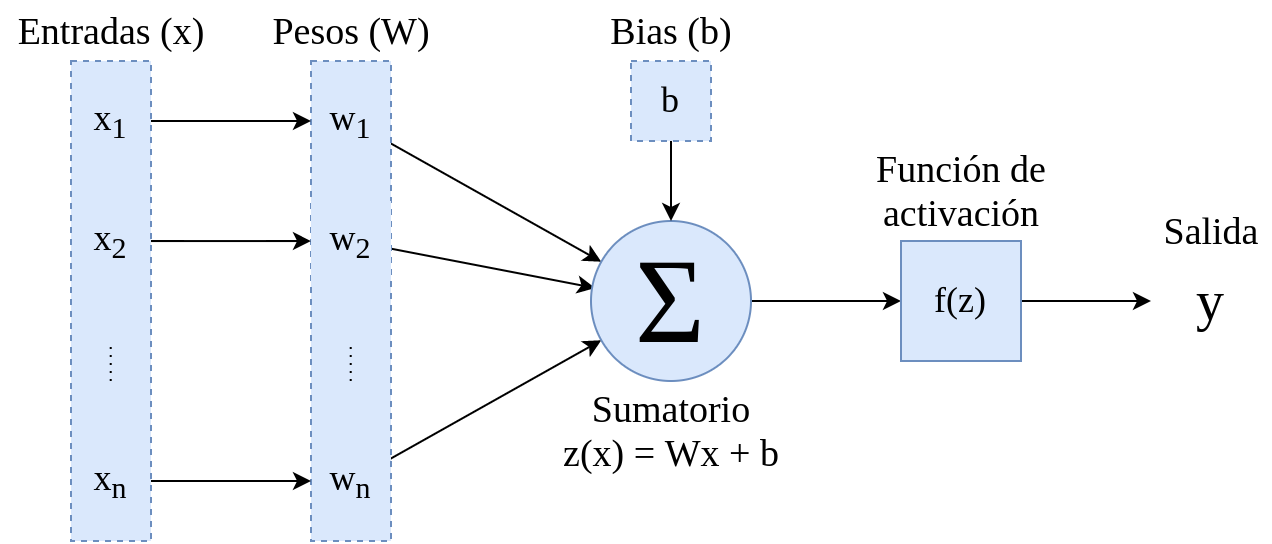
\includegraphics[width=.75\linewidth]{imagenes/neurona.png} 
\captionsetup{width=.5\linewidth}
\caption{Estructura de una neurona artificial.}
\label{fig:neurona}
\end{figure}

Una de las bases teóricas más importantes de las NN, es que con un conjunto de neuronas lo suficientemente grande y funciones de activación no lineales, es posible aproximar cualquier función continua (\textit{Universal approximation theorem} \cite{universal-approximators}). Por desgracia, ajustar los parámetros (pesos y bias) de cada una de las neuronas de dicha red para aproximar la función deseada no es un problema trivial. 

Una de las soluciones más comunes a este problema, es, de forma iterativa, modificar los parámetros de forma que minimicen la distancia entre la salida de la red y la función que se busca aproximar. Para esto, se emplea la propagación hacia atrás (\textbfit{backpropagation}) \cite{backprop}, que necesita: un \textbf{optimizador} (en los que se profundiza más adelante), un \textbf{conjunto de entradas con salidas conocidas} y una \textbf{función de perdida} que se emplea como aproximación optimizable de la distancia previamente mencionada. Este algoritmo, de forma simplificada, consiste en:

\begin{enumerate}
\item Calcular la salida de la red a partir de las entradas de las cuales conocemos la salida esperada (\textbfit{forward pass}).
\item Emplear una \textbf{función de pérdida} para calcular una medida del error entre la salida obtenida y la salida esperada.
\item Calcular las derivadas parciales del error respecto de cada uno de los parámetros (\textbf{pesos} y \textbfit{bias}) que se quieren ajustar.
\item Ajustar los valores de los parámetros en función de su influencia en el error empleando un optimizador concreto.
\end{enumerate}

Estos pasos, normalmente se repiten varias veces para cada ejemplo disponible (entendiendo como ejemplo las parejas entrada-salida conocidas). En el contexto de las redes neuronales, este proceso de ajuste se conoce como \textbf{entrenamiento} y cada una de las iteraciones que la red realiza sobre el conjunto de ejemplos se conoce como \textbf{época} (\textit{epoch}, en inglés). 

El proceso de entrenamiento, sin embargo, hay que controlarlo y validarlo de alguna forma, ya que existe el riesgo de sobreajustar los parámetros de la red neuronal a los datos de entrenamiento, siendo el modelo incapaz de generalizar a datos no antes vistos. Este sobreajuste se conoce en inglés como \textbfit{overfitting}. Para controlar si el modelo se está sobreajustando, es común dividir el conjunto de datos en tres subconjuntos: entrenamiento, validación, y evaluación. El conjunto de entrenamiento, se emplea para ajustar los parámetros del modelo; el de evaluación, para comprobar si hay \textit{overfitting} y para elegir entre distintas configuraciones de un mismo modelo o distintos modelos; y el de evaluación, para calcular las métricas finales del modelo elegido para un problema concreto. En el trabajo de Sebastian Raschka \cite{model-evaluation} se presentan distintas formas de hacer estas particiones, en este trabajo, no obstante, se emplearán particiones ya establecidas en la literatura existente para los conjuntos de datos empleados (\Cref{conjuntos-kitti}).

A continuación, se profundiza en algunos de los conceptos mencionados prestando especial atención a los elementos que aparecen en este trabajo.

\subsubsection{Funciones de activación}
Tal y como se ha visto en la \Cref{fig:neurona}, la función de activación transforma la suma del \textit{bias} y el producto de los pesos y las entradas para obtener el valor de salida. En la \Cref{fig:funciones-activacion}, es posible observar graficadas varias de estas funciones junto con sus ecuaciones.

\begin{figure}[H]
\centering
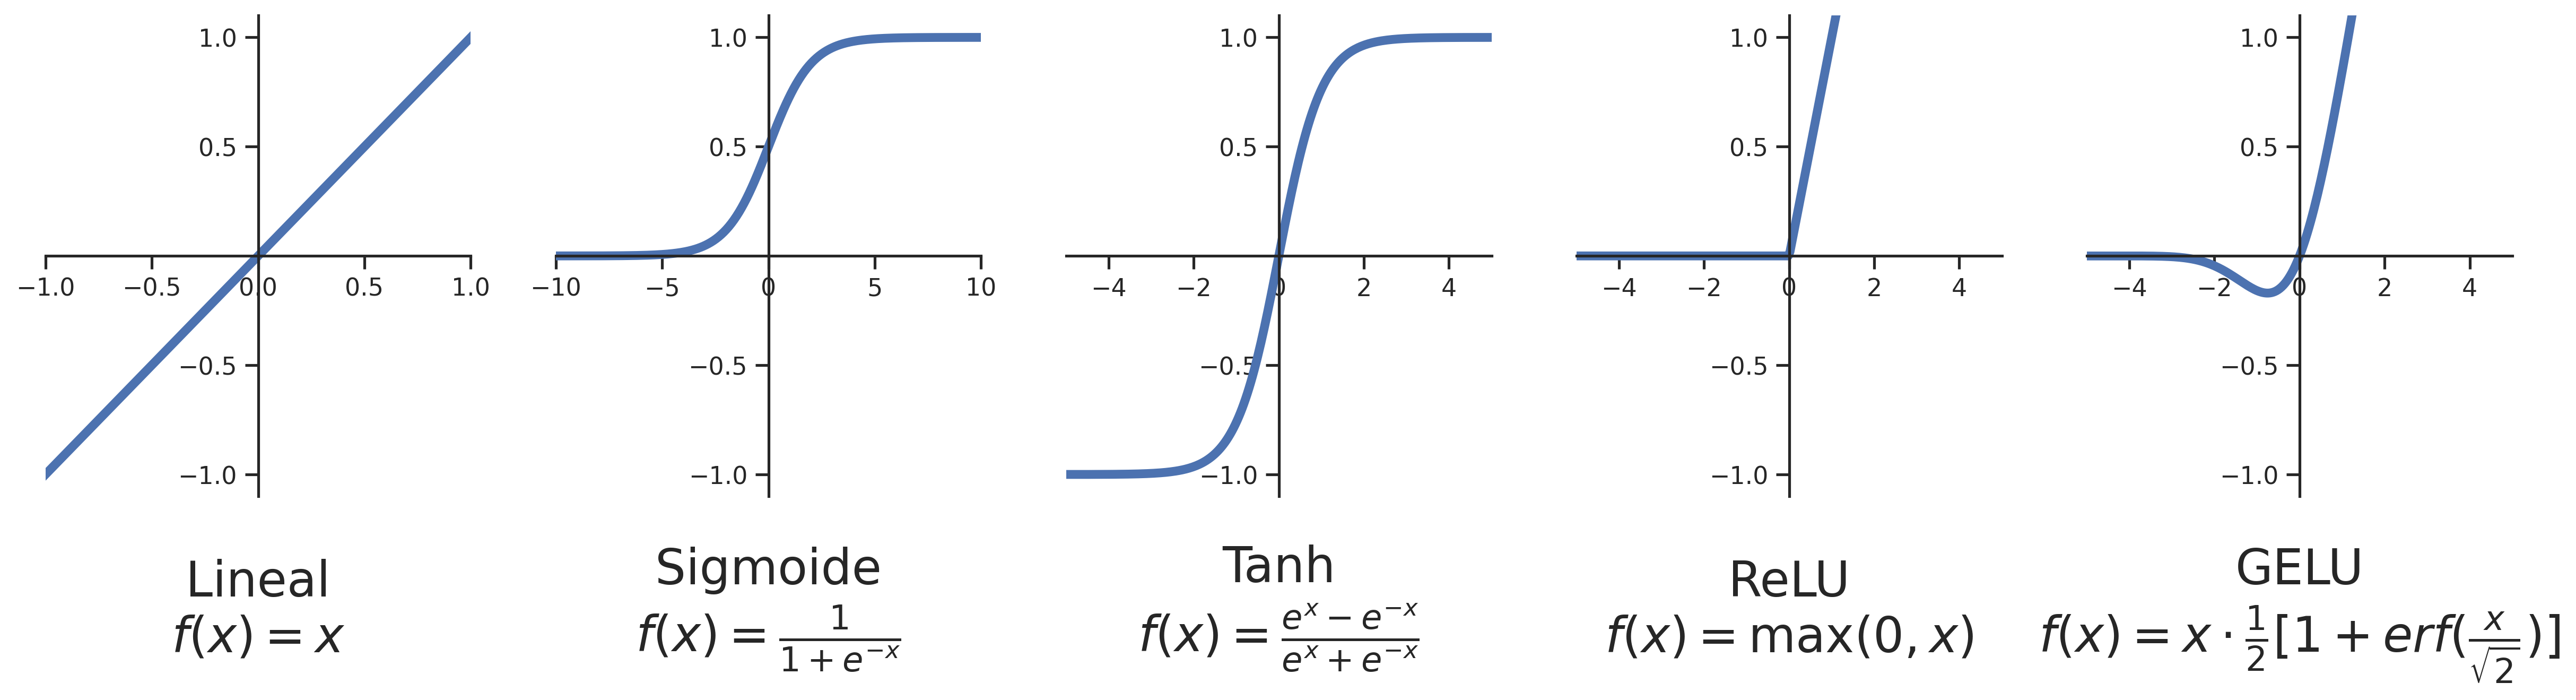
\includegraphics[width=\linewidth]{imagenes/funciones_activacion.png} 
\captionsetup{width=.8\linewidth}
\caption{Funciones de activación.}
\label{fig:funciones-activacion}
\end{figure}

La primera de estas funciones de activación es la función de activación lineal. Esta función, no suele emplearse, ya que al concatenar múltiples neuronas con activaciones lineales, se obtiene otra función lineal que podría representarse con una sola neurona. Por esta razón, son funciones no lineales como la sigmoide, la tangente hiperbólica, ReLU (\textit{Rectified Linear Unit}) \cite{relu} o GELU (\textit{Gaussian Error Linear Unit}) \cite{gelu} las que suelen aparecer en las arquitecturas actuales. 

Cada una de estas funciones de activación tiene características propias que las hacen diferentes entre si. La tangente hiperbólica, aún siendo similar a la sigmoide, es simétrica y tiene unos gradientes más fuertes en las zonas cercanas al cero, lo que origina que sus salidas sean valores pequeños centrados en cero y que el entrenamiento sea más rápido \cite{lecun2012efficient}. La función ReLU, por otro lado, pese a ser parcialmente lineal, puede aproximar funciones no lineales gracias a su definición a trozos, además, el gradiente para los valores positivos es constante $(1)$, reduciendo en gran medida el desvanecimiento de los gradientes cuando se definen redes neuronales con un gran número de capas. Por último, la función GELU, es comúnmente empleada en las arquitecturas basadas en \textit{transformers} y mantiene el gradiente constante en valores positivos a la vez que añade una ligera ponderación a los valores negativos cercanos al cero.

\subsubsection{Funciones de pérdida}
Las funciones de pérdida, tal y como se ha mencionado previamente, son aproximaciones optimizables de la distancia o error entre el valor real a predecir y la predicción realizada. Dentro de estas funciones, cuyo valor se busca minimizar, existen diferentes situaciones que pueden dificultar el aprendizaje de los modelos, por ejemplo, los mínimos locales, donde los valores de la función de pérdida son menores que los valores de su entorno, originando que los gradientes se desvanezcan y detengan el proceso de optimización, o los puntos de silla (\textit{saddle points}), donde, pese a no haber un mínimo local, los gradientes también se desvanecen, deteniendo la minimización.

\subsubsection{Optimizadores}
Los optimizadores son algoritmos que minimizan el valor de la función de pérdida ($f(\theta)$) ajustando los parámetros ($\theta$) de los modelos, entre otras cosas, en base a la influencia de estos parámetros en el error obtenido en dicha función. Esta influencia se obtiene calculando las derivadas parciales del error respecto de cada parámetro (gradiente: $\nabla_{\theta} f_t(\theta_{t-1})$), y, en función del algoritmo que se elija, puede verse afectada por distintos factores. Algunos de los optimizadores más empleados son SGD, AdaGrad \cite{adagrad}, RMSProp \cite{rmsprop} TODO, Adam \cite{adam} o AdamW \cite{adamw}.

El descenso de gradiente tradicional promedia los gradientes del error en todos los ejemplos disponibles para actualizar los parámetros. La modificación que introduce el \textbf{SGD (\textit{Stochastic Gradient Descent})}, es actualizar los parámetros tras ver cada uno de los ejemplos. De esta forma, se acelera el entrenamiento, ya que aunque cada ajuste no es óptimo, los parámetros se actualizan mucho más frecuentemente. Además, el ruido intrínseco de cada ejemplo tiene un efecto regularizador que puede ayudar a salir de mínimo locales.

No obstante, gracias a la capacidad de procesamiento paralelo de las tarjetas gráficas es muy común promediar el cálculo del error en pequeños subconjuntos (\textbfit{batch}) de todos los datos disponibles. Esto se conoce como \textit{Mini Batch Gradient Descent} y el tamaño (\textbfit{batch size}) que se elija influye directamente en diferentes factores como son la velocidad de entrenamiento, la rapidez para converger, o el punto al que se converge \cite{on-large-batch}.

Estos tres algoritmos, y en general la mayoría de los optimizadores, controlan el cambio de los parámetros mediante un hiperparámetro conocido como tasa de aprendizaje (\textit{learning rate}: $\gamma$), que se multiplica por el valor del gradiente de la función de pérdida respecto de los parámetros (\Cref{eqn:sgd}).

\begin{equation}
\label{eqn:sgd}
\theta_t = \theta_{t-1} - \gamma (\nabla_{\theta} f_t(\theta_{t-1}))
\end{equation}

En el caso del \textit{Mini Batch Gradient Descent}, al promediar los gradientes de varios ejemplos se reduce el ruido del SGD. Inspirado por el concepto físico de \textbf{Momento}, es posible añadir a estos optimizadores una modificación para que se consideren también los gradientes de los pasos anteriores del optimizador. De esta forma, se reduce el ruido y se hace más robusta la optimización frente a mínimos locales. El momento se controla con un hiperparámetro $\mu$ siguiendo la \Cref{eqn:momento}, donde $v_t$ es el Momento en un paso concreto y $g_{t, t-1}$ los gradientes correspondientes a este paso. 

\begin{equation}
\label{eqn:momento}
v_t = \mu v_{t-1} + g_{t, t-1}
\end{equation}

Este cálculo multiplica los momentos anteriores de forma recursiva por un valor menor que uno, de forma que influyen todos los gradientes anteriores, pero cada vez con menos fuerza. Esto se puede ver comprobar matemáticamente desarrollando la \Cref{eqn:momento} (\Cref{eqn:momento2}). Finalmente, este momento toma la posición del gradiente en la actualización de los parámetros (\Cref{eqn:momento3}).

\begin{equation}
\label{eqn:momento2}
v_t = \mu^2 v_{t-2} + \mu g_{t-1, t-2} + g_{t, t-1} = \sum_{i=0}^{t-1}\mu^{i}g_{t-i, t-i-1}
\end{equation}
\begin{equation}
\label{eqn:momento3}
\theta_t = \theta_{t-1} - \gamma (v_t)
\end{equation}

\textbf{AdaGrad (\textit{Adaptative Gradients})} es otro optimizador que también modifica el descenso del gradiente. En este caso, para reducir las tasas de aprendizaje en aquellos parámetros que han tenido mayores derivadas parciales, dividiendolas entre la suma de los gradientes ($g$) anteriores (\Cref{eqn:adagrad} y \Cref{eqn:adagrad2}). Estos gradientes se acumulan durante toda la optimización, por lo que es especialmente efectivo en datos dispersos donde no en todos los ejemplos se dispone de todas las características, ya que las características que no se hayan visto tan frecuentemente, tendrán actualizaciones mayores. Esto, sin embargo, también ralentiza el algoritmo, ya que según avanza el proceso, las actualizaciones de los parámetros son menores y pueden llegar a detener el proceso, impidiendo que se alcance a un mínimo aceptable.

\begin{equation}
\label{eqn:adagrad}
acumulaci\acute{o}n_t = acumulaci\acute{o}n_{t-1} + g^{2}_{t}
\end{equation}
\begin{equation}
\label{eqn:adagrad2}
\theta_t = \theta_{t-1} - \gamma \frac{g_t}{\sqrt{acumulaci\acute{o}n_t}}
\end{equation}

% https://towardsdatascience.com/a-visual-explanation-of-gradient-descent-methods-momentum-adagrad-rmsprop-adam-f898b102325c

\textbf{RMSProp (\textit{Root Mean Square Propagation})} soluciona el problema de la velocidad de AdaGrad añadiendo un factor de decaimiento. Este factor de decaimiento (\textit{decay rate}: $\alpha$), escala de forma recursiva la suma acumulada de los gradientes anteriores (media movil exponencialmente ponderada - \textit{Exponential weighted moving averages}), por lo que a medida que el optimizador avanza, la influencia de los gradientes anteriores disminuye. De esta forma, se mantienen los beneficios de AdaGrad evitando reducir indefinidamente la magnitud de la actualización de los parámetros (\Cref{eqn:RMSProp} y \Cref{eqn:RMSProp2}).

\begin{equation}
\label{eqn:RMSProp}
acumulaci\acute{o}n_t = (\alpha) acumulaci\acute{o}n_{t-1} + (1-\alpha) g^{2}_{t}
\end{equation}
\begin{equation}
\label{eqn:RMSProp2}
\theta_t = \theta_{t-1} - \gamma \frac{g_t}{\sqrt{acumulaci\acute{o}n_t}}
\end{equation}

Por último, \textbf{Adam} y \textbf{AdamW} son dos optimizadores que fusionan las ideas y ventajas detrás del momento y de RMSProp. Para conseguir esto, se vuelve a aplicar la media móvil exponencialmente ponderada, esta vez tanto para el primer como el segundo momento, controlado por dos parámetros $\beta$ (\Cref{eqn:Adam} y \Cref{eqn:Adam2}).

\begin{equation}
\label{eqn:Adam}
m_t = \beta_1 m_{t-1} + (1-\beta_1) g_{t}
\end{equation}
\begin{equation}
\label{eqn:Adam2}
v_t = \beta_2 v_{t-1} + (1-\beta_2) g^{2}_{t}
\end{equation}

Además, para reducir la influencia del valor inicial (igual a cero) de $m_0$ y $v_0$, se añade una normalización que sigue la \Cref{eqn:Adam3} y la \Cref{eqn:Adam4}.

\begin{equation}
\label{eqn:Adam3}
\hat{m}_t = \frac{m_t}{(1-\beta^{t}_{1})}
\end{equation}
\begin{equation}
\label{eqn:Adam4}
\hat{v}_t = \frac{v_t}{(1-\beta^{t}_{2})}
\end{equation}

Una vez calculados estos dos términos, se actualizan los parámetros de forma similar a como se hacía en RMSProp, con la diferencia de que esta vez se multiplica por el momento acumulado y no por los gradientes (\Cref{eqn:Adam5}).

\begin{equation}
\label{eqn:Adam5}
\theta_t = \theta_{t-1} - \gamma \frac{\hat{m}_t}{\sqrt{\hat{v}_t}}
\end{equation}

En cuanto a la diferencia entre Adam y AdamW, esta reside en cómo se implementa el \textit{weight decay}, un tipo de regularización que penaliza los pesos mayores ya que pueden introducir mayor varianza en el modelo (\textit{overfitting}). Tal y como se indica en el artículo \textit{Decoupled Weight Decay Regularization} \cite{adamw}, la implementación del \textit{weight decay} en los optimizadores (Adam entre ellos) aplica este decaimiento en los gradientes. Sin embargo, al añadir las operaciones relacionadas con los gradientes adaptativos, aplicar el decaimiento en los gradientes deja de ser equivalente a aplicarlo realmente en los pesos. AdamW soluciona este problema implementando el método de regularización correctamente.

% https://stackoverflow.com/questions/64621585/adamw-and-adam-with-weight-decay
% https://www.fast.ai/2018/07/02/adam-weight-decay/
% https://towardsdatascience.com/weight-decay-l2-regularization-90a9e17713cd
% https://towardsdatascience.com/why-adamw-matters-736223f31b5d

\subsection{MLP}
El Perceptrón Multicapa, o por sus sigles en ingles, \textbf{MLP} (\textit{Multi Layer Perceptron}), es una de las arquitecturas de red neuronal más básicas y está formado por una capa de entrada, una capa de salida, y un bloque de capas intermedias u ocultas. Estas capas intermedias, son agrupaciones de neuronas donde cada una de las neuronas (normalmente) se conecta con todas las neuronas de la capa anterior y con todas las neuronas de la capa posterior (\Cref{fig:mlp}). De esta forma, se crea una sucesión donde las entradas de una neurona son las salidas de las neuronas de la capa anterior y la salida de dicha neurona es una de las entradas de todas las neuronas de la capa siguiente. 

\begin{figure}[H]
\centering
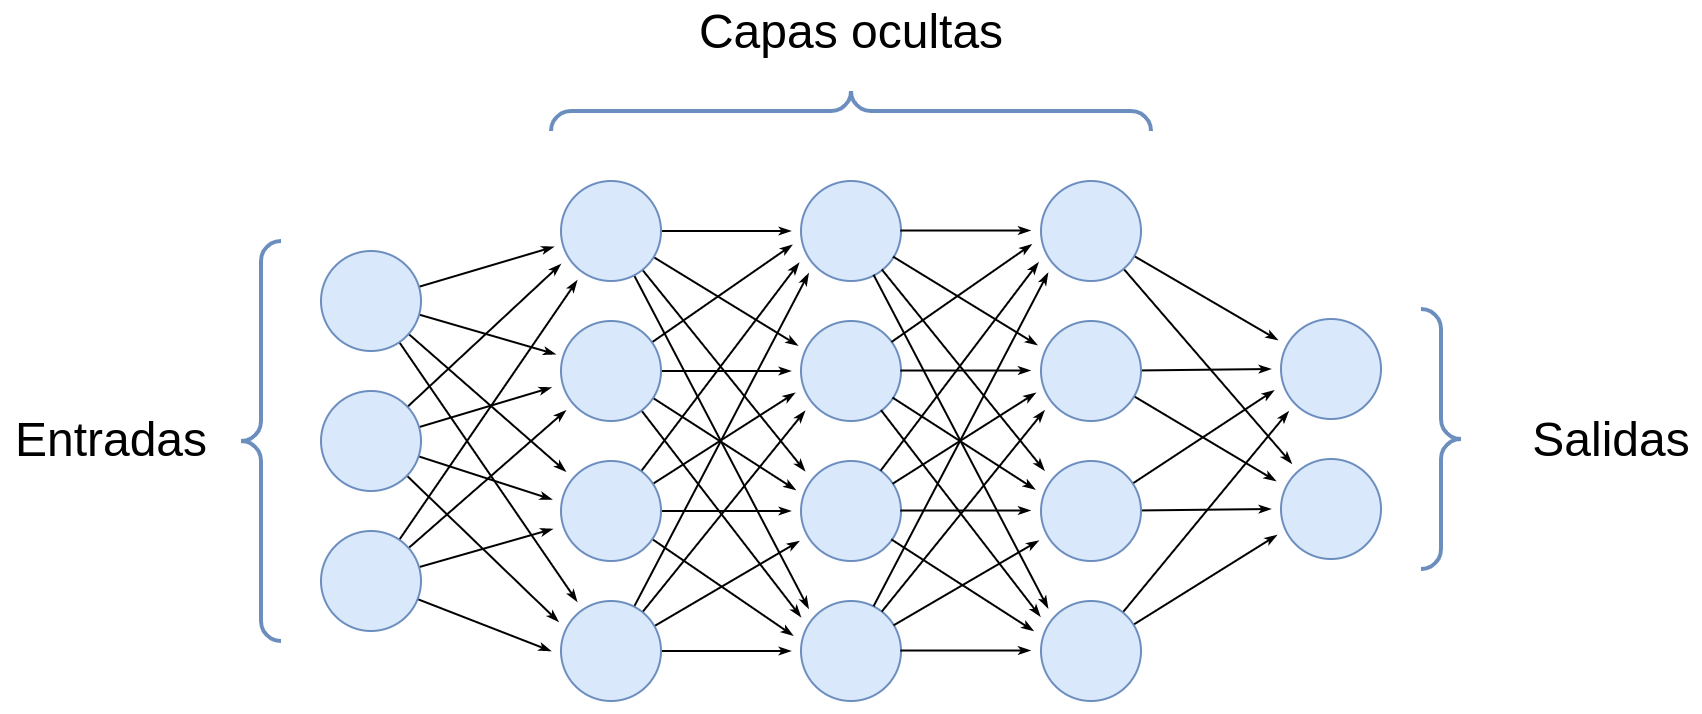
\includegraphics[width=0.8\linewidth]{imagenes/mlp.png} 
\captionsetup{width=.8\linewidth}
\caption{Perceptrón Multicapa.}
\label{fig:mlp}
\end{figure}

\subsection{RNN}
Las redes neuronales recurrentes (\textit{Recurrent Neural Networks} - RNN) son un grupo de redes neuronales cuya arquitectura se fundamenta en la utilización repetida de la salida de la propia red en un instante como entrada adicional de la red en el instante siguiente. Para conseguir esto, se mantiene la información en forma de estado oculto (\textit{hidden state}). Gracias a esta transmisión recurrente, es posible transferir información entre entradas sucesivas de la red.

Este tipo de redes está especialmente diseñado para trabajar con entradas secuenciales de valores (series temporales, texto, señales de audio y video, etc.) ya que su arquitectura aprovecha la información de los datos previos y no tiene limitaciones en el tamaño de la secuencia de entrada.

Sin embargo, la ejecución y entrenamiento de este tipo de redes requiere ejecutarlas individualmente con cada uno de los valores de la entrada, haciendo que el proceso sea temporalmente costoso. Además, pese a que se han presentado distintas modificaciones como las celdas GRU (\textit{Gated Recurrent Units}) \cite{cho-etal-2014-learning} o LSTM (\textit{Long Short-Term Memory}) \cite{HochSchm97} que los mitigan, también sufren tanto de desvanecimientos de gradientes por las activaciones sucesivas como de pérdida de información en cadenas de gran tamaño (al codificar toda la información anterior en un estado oculto, llega un punto en el que la información almacenada en instantes alejados temporalmente deja de ser representativa).

\begin{figure}[H]
\centering
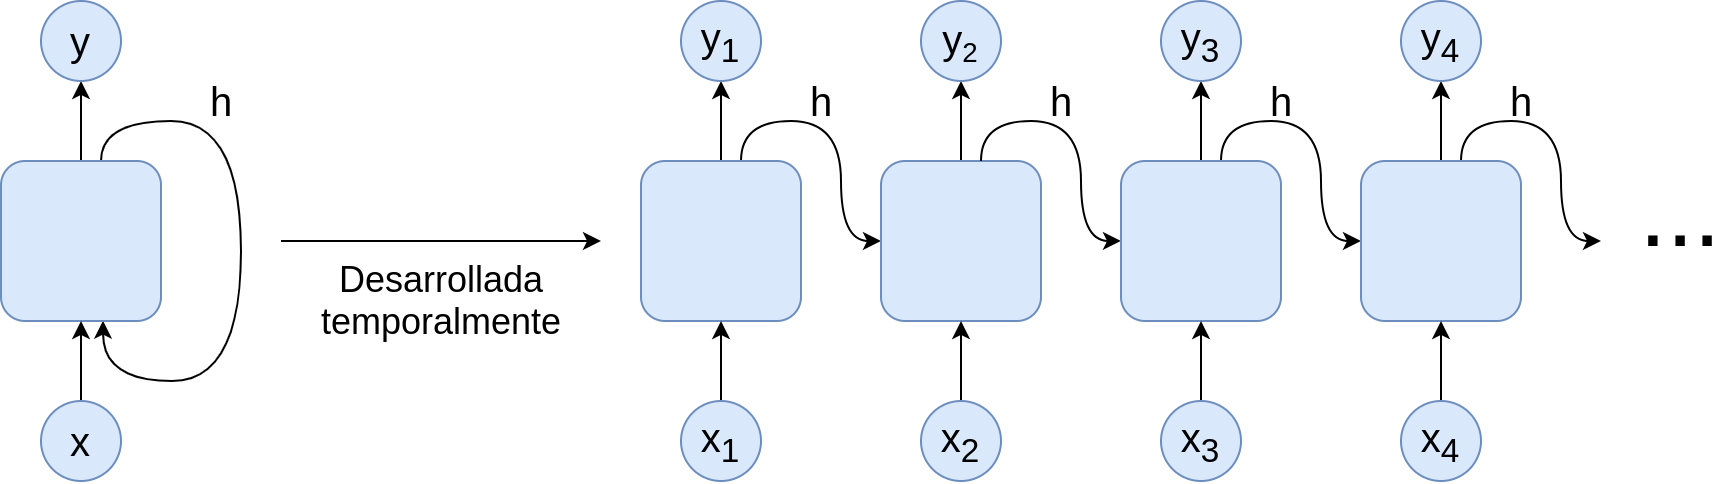
\includegraphics[width=0.8\linewidth]{imagenes/rnn.png} 
\captionsetup{width=.8\linewidth}
\caption{Red recurrente.}
\label{fig:rnn}
\end{figure}

\subsection{CNN}
A la hora de trabajar con imágenes (matrices de dos o tres dimensiones), el número de conexiones, y por lo tanto, parámetros, que tendrían que existir para conectar cada valor de entrada con cada neurona crece enormemente. Las redes convolucionales, no solo lidian con este problema, si no además lo hacen proporcionando muy buenos resultados. Este tipo de redes, se basan en el concepto de núcleo (\textit{kernel}) proveniente del procesamiento digital de imágenes y la operación de convolución, y su origen se atribuye al trabajo de LeCun et al. \cite{LeCun1999}.

Los filtros o \textit{kernels} (\Cref{fig:convolucion}) son pequeñas matrices (cuyos valores son equivalentes a los pesos vistos anteriormente, y por lo tanto son ajustados durante el entrenamiento) que se convolucionan sobre la imagen de entrada, extrayendo de esta forma mapas de características (también conocidos como mapas de activaciones) que son a su vez la entrada de las siguientes capas convolucionales tras aplicar una función de activación y puede que otras operaciones. En cuanto a la convolución (o correlación cruzada\footnote{La operación matemática de convolución entre dos funciones incluye voltear una de las funciones. Sin embargo, en el campo del Deep Learning, voltear la entrada o el filtro requeriría una operación adicional que solo conllevaría que los pesos obtenidos tras el descenso de gradiente estuvieran también volteados. Por lo tanto, la operación de convolución en redes neuronales realmente es una operación de correlación cruzada donde no se voltea ninguna de las funciones.}), es una operación cuya salida se obtiene desplazando una de las dos matrices y calculando su producto escalar con la otra matriz (\Cref{fig:convolucion}). Estas capas, están definidas principalmente por el tamaño del \textit{kernel}, el número de \textit{kernels} que se aplican y la zancada o \textit{stride}, que es el desplazamiento del \textit{kernel} para calcular cada valor de salida y por lo tanto afecta directamente en su tamaño. 

\begin{figure}[H]
\centering
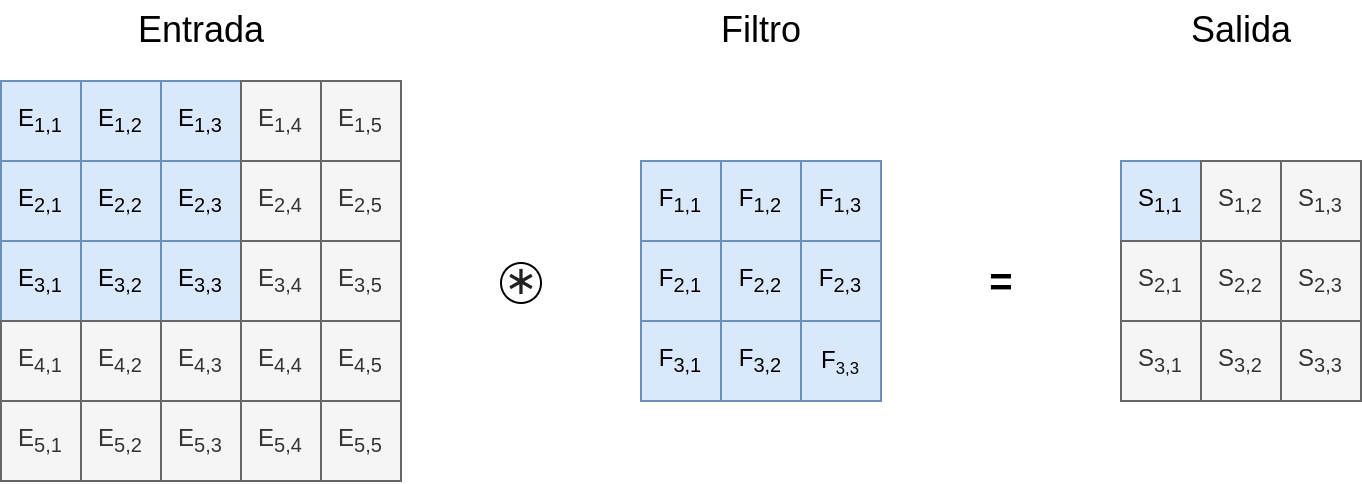
\includegraphics[width=0.8\linewidth]{imagenes/convolucion.png} 
\captionsetup{width=.8\linewidth}
\caption{Operación de convolución con un \textit{kernel} de $3\times3$ y un \textit{stride} de $1$ para uno de los valores de salida.}
\label{fig:convolucion}
\end{figure}

Los \textit{kernels}, normalmente tienden a extraer características de más alto nivel cuanto más adelante están en la red. Esto significa que los mapas de características resultantes en las capas iniciales son características de muy bajo nivel (lineas verticales, horizontales, curvas, esquinas, etc.), mientras que las de las últimas capas extraen características más complejas propias de cada dominio de aplicación \cite{zeiler2014visualizing}.

En las redes convolucionales, es común encontrar otras operaciones como son:
\begin{itemize}
\item Pooling: Las capas de \textit{Pooling} se emplean principalmente para reducir el tamaño de los mapas de características resultantes de las capas convolucionales. Para conseguirlo, agrupan un conjunto de valores en un solo valor aplicando una función que normalmente es el máximo (\textit{MaxPooling} - se escoge el máximo valor) o la media (\textit{AveragePooling} - se calcula la media de los valores). La operación de \textit{Pooling} está definida principalmente por dos valores similares a los de la convolución: el tamaño del \textit{kernel}, que define el tamaño del subconjunto de valores; y la zancada o \textit{stride}, que define el número de valores que se traslada el \textit{kernel} cada paso. En la \Cref{fig:pooling}, se puede observar una operación de \textit{Pooling} con un \textit{kernel} y un \textit{stride} de $2\times2$ donde cada uno de los valores de la salida se calcula a partir de los valores de la entrada con el mismo color.

\begin{figure}[H]
\centering
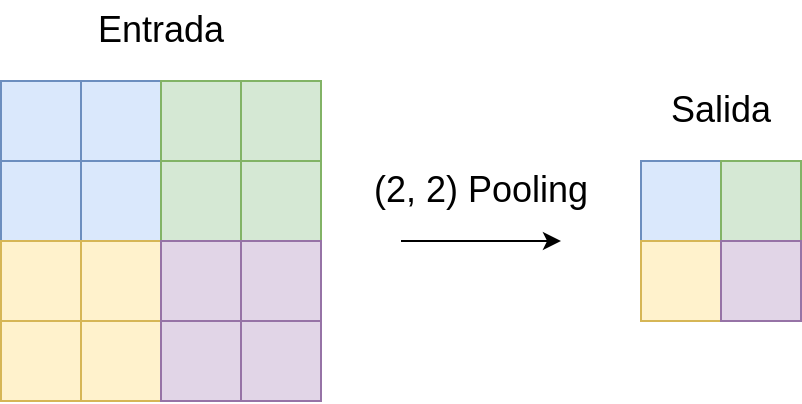
\includegraphics[width=0.5\linewidth]{imagenes/pooling.png} 
\captionsetup{width=.5\linewidth}
\caption{Operación de Pooling2D.}
\label{fig:pooling}
\end{figure}

\item Convolución transpuesta: La operación de convolución puede, dependiendo del tamaño del \textit{kernel}, producir un resultado de dimensiones espaciales (altura y anchura) iguales o menores que las de la entrada. Sin embargo, para obtener una salida con mayores dimensiones que la entrada es necesario recurrir a la convolución transpuesta, una operación similar a la convolución donde para obtener los valores de la salida, se multiplican todos los valores del \textit{kernel} por solo uno de los valores de la entrada, que se recorren individualmente. Al hacer el cálculo de esta forma, dependiendo de la zancada (\textit{stride}) que se elija, pueden solaparse valores de la salida, por lo que se suman aquellos que hayan obtenido un valor en más de una operación (\Cref{fig:transpose}).

\begin{figure}[H]
\centering
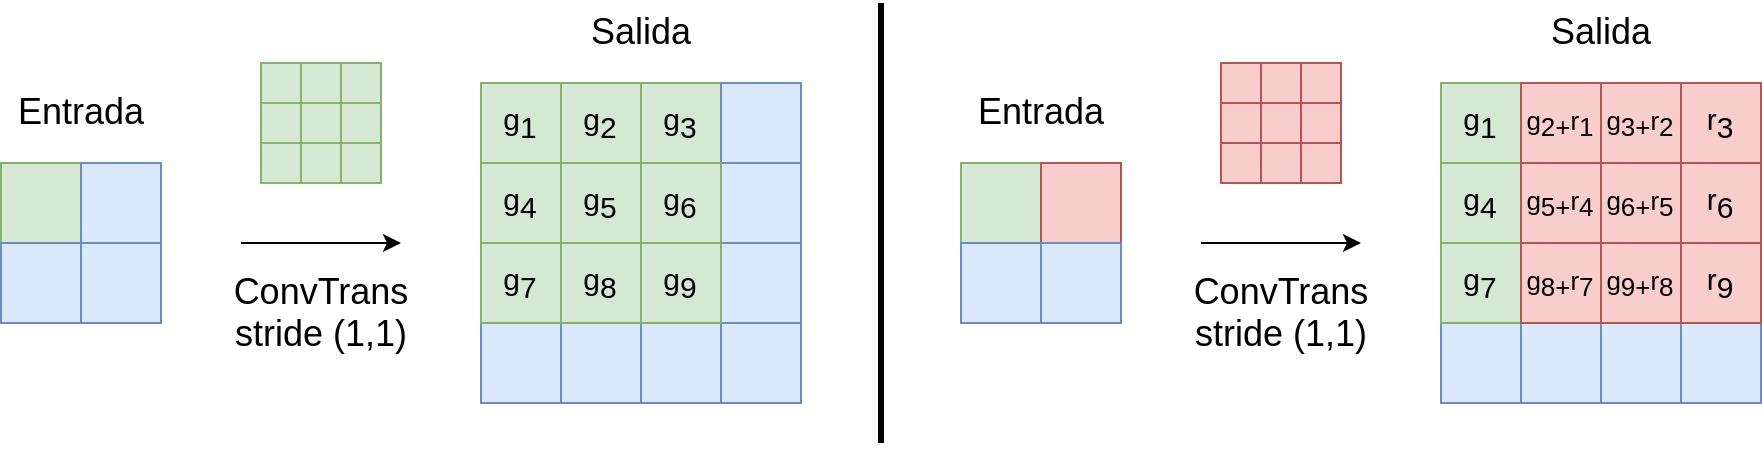
\includegraphics[width=0.9\linewidth]{imagenes/transpose-convolution.png} 
\captionsetup{width=.75\linewidth}
\caption{Primeros pasos de una convolución transpuesta.}
\label{fig:transpose}
\end{figure}

\item Convolución 1x1 (\textit{Pointwise Convolution}): Pese a que no es un tipo de capa distinta per se, esta aplicación particular de la convolución suele emplearse junto a otro tipo de capas o como proyección para modificar el número de canales. Su principio de funcionamiento es el uso de \textit{kernels} de tamaño $1\times1$ y tantos canales como mapas de características tenga la entrada. De esta forma, cada uno de los filtros produce un solo canal de igual altura y anchura que la entrada en la salida, permitiendo por lo tanto controlar con el número de filtros de la capa convolucional el nuevo número de canales en el que se proyecta la entrada (\Cref{fig:convolucion1x1}).

\begin{figure}[H]
\centering
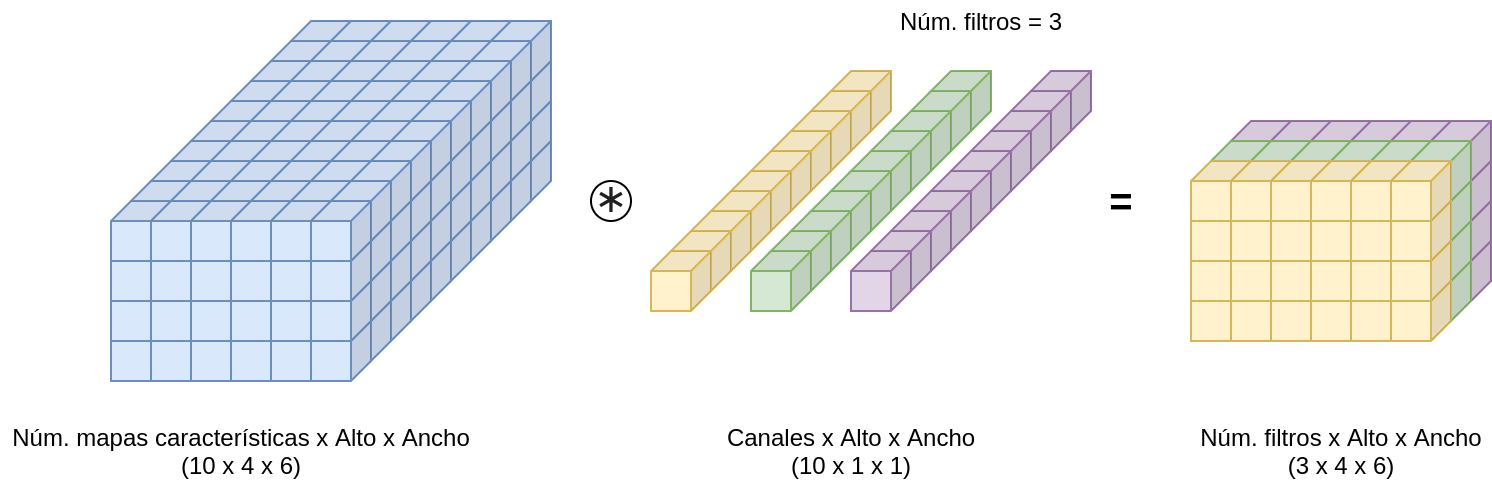
\includegraphics[width=0.9\linewidth]{imagenes/convolucion1x1.png} 
\captionsetup{width=.9\linewidth}
\caption{\textit{Pointwise convolution}.}
\label{fig:convolucion1x1}
\end{figure}

\item Convolución por profundidad separable (\textit{Depthwise Separable Convolution}): Similar al caso anterior, este cálculo es mas bien un caso especial de la capa de convolución. La operación de convolución por profundidad separable se compone de dos partes: 

\begin{enumerate}
\item Una convolución por profundidad donde los \textit{kernels} solamente tienen un canal y se aplican de forma individual en solo uno de los canales (el número de \textit{kernels} tiene que ser igual al número de canales en la entrada) para luego agrupar los resultados (\Cref{fig:convolucion-depthwise}).
\item Una convolución con un solo \textit{kernel} de tamaño $1\times1$, fusionando los canales individuales resultantes de la operación anterior en uno solo. De esta forma, la operación se asemeja a una convolución corriente en la que el \textit{kernel} tendría tantos canales como la entrada, pero reduciendo muy considerablemente el número de operaciones.
\end{enumerate}

\begin{figure}[H]
\centering
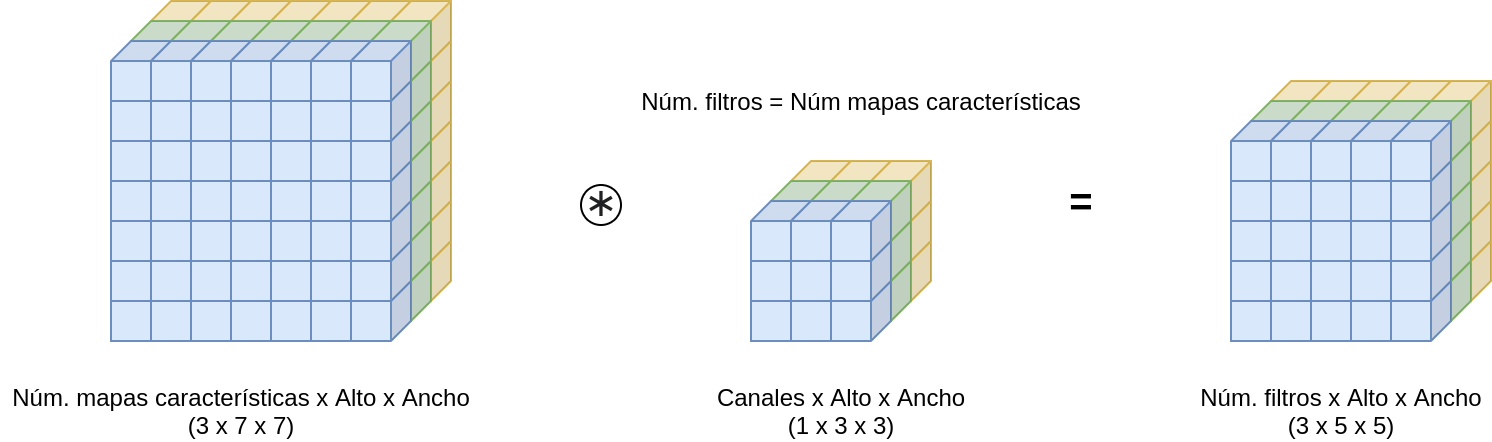
\includegraphics[width=0.9\linewidth]{imagenes/convolucion-depthwise.png} 
\captionsetup{width=.9\linewidth}
\caption{\textit{Depthtwise convolution}.}
\label{fig:convolucion-depthwise}
\end{figure}

\end{itemize}

\subsubsection{Conexiones residuales y ResNets}

En el artículo publicado por He et al. \cite{resnet} se presentan las conexiones residuales y la familia de redes ResNet, compuesta por distintos modelos en función de su número de capas. En el momento en el que se publicó dicho estudio, gracias a las conexiones residuales, se consiguió multiplicar por aproximadamente $7$ el número de capas en los modelos del estado del arte (de las 22 capas de GoogleLeNet \cite{googlelenet} a las 152 capas de ResNet152). Para conseguir esto, las ResNet se apoyan en las conexiones residuales (\Cref{fig:residual}), que permiten aumentar tanto la capacidad de aprendizaje de las redes como la calidad de sus resultados.

\pagebreak

\begin{wrapfigure}{r}{0.4\textwidth}
\vspace{-5pt}
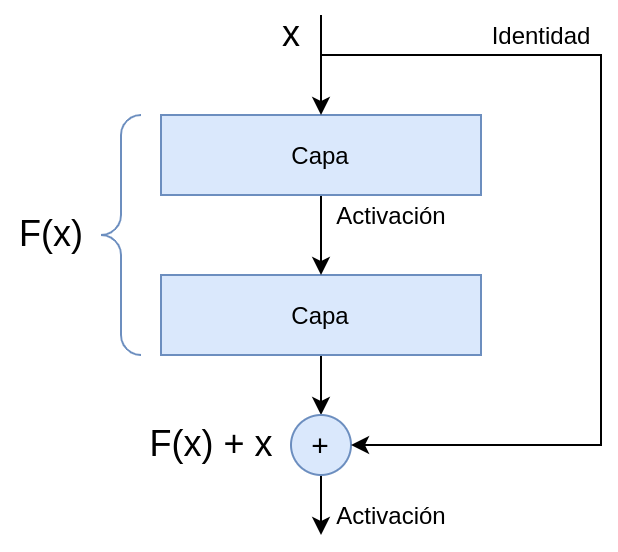
\includegraphics[width=0.95\linewidth]{imagenes/residual-connection.png} 
\caption{Conexión residual básica.}
\label{fig:residual}
\end{wrapfigure}

Las conexiones residuales están motivadas por la idea de que dada una red con una profundidad óptima para una tarea, en teoría, por muchas capas que se incluyesen, el descenso del gradiente sería capaz de hacer que las capas adicionales convergiesen en una función identidad y no perjudicasen los resultados. No obstante, empíricamente se ha comprobado que con las redes neuronales llega un punto en el que añadir más profundidad hace que los resultados empeoren. Aquí es donde entran las conexiones residuales, ya que al pasar hacia adelante la entrada de un bloque de capas y sumarlo a su salida (\Cref{fig:residual}), se facilita que el descenso del gradiente reste importancia a la señal que ha atravesado dicho bloque ($F(x)$) en caso de que no mejore la salida final de la red.

Además, para reducir el uso de recursos computacionales al incrementar el número de capas, las ResNet utilizan conexiones residuales con cuellos de botella (\textit{bottleneck}) para reducir el tiempo de ejecución. Este sistema, en vez de usar como $F(x)$ (\Cref{fig:residual}) dos capas convolucionales, emplea tres, siendo la primera y la tercera convoluciones de filtros $1\times1$ que se encargan de reducir el número de canales y posteriormente incrementarlo para que se pueda sumar con la entrada. De esta forma, se reducen en gran medida el número de operaciones a realizar en la capa convolucional central, con filtros de tamaño $3\times3$. 

% Aunque se supone que es resnetv2, https://github.com/rwightman/pytorch-image-models/blob/b669f4a5881d17fe3875656ec40138c1ef50c4c9/timm/models/resnetv2.py#L194 en ViT no se usa el bloque con preactivación.


\subsubsection{EfficientNet}
Otro conjunto de arquitecturas, es el presentado en el artículo \textit{EfficientNet: Rethinking Model Scaling for Convolutional Neuronal Networks} \cite{efficientnet}, que propone un método para escalar de forma proporcional la profundidad (número de capas), anchura (número de filtros) y resolución de entrada de las redes convolucionales de forma que se puedan adaptar los modelos a los recursos disponibles. En esta publicación, se presenta la red \textbf{EfficientNet-B0} (inicialmente diseñada para ilustrar el escalado proporcional propuesto) y su familia de redes, que se obtienen escalando dicho modelo. Sin embargo, más allá de ilustrar el escalado en anchura, profundidad y resolución, la arquitectura de la familia de EfficientNets obtiene resultados muy competitivos con un número de parámetros muy reducido en comparación con el de sus competidores.

Para diseñar esta red se extiende el trabajo de Tan et al. \cite{mnasnet}, y se emplea \textit{Neural Architecture Search - NAS} (una técnica que automatiza la búsqueda y configuración de arquitecturas de redes neuronales) buscando optimizar el \textit{accuracy} \todo{En español exactitud me suena feo y precisión me suena a precision} y el número de operaciones en coma flotante (FLOPS). Como resultado, se obtiene una arquitectura basada en bloques de capas MBConv (\textit{Mobile Inverted Bottleneck Residual Convolution}) \cite{mobilenetv2} y \textit{Squeeze-and-Excitation} \cite{senet}.

La primera de estas dos capas, (MBConv) se propone en la publicación de \textbf{MobileNetV2} \cite{mobilenetv2} y modifica los bloques con conexiones residuales y cuello de botella inviertiendolos. En vez de utilizar filtros de $1\times1$ para reducir el número de mapas de características y después aumentarlo, este bloque emplea dichos filtros para aumentar y luego reducir el número de canales. Sin embargo, emplea convoluciones por profundidad separables (\textit{Depthwise Separable Convolutions}) para reducir enormemente el número de operaciones al aumentar el número de canales. 

La segunda, es uno de los bloques principales de la \textbf{SENet} \cite{senet} y basa su funcionamiento en dos operaciones que realmente pueden añadirse a cualquier otra capa: el mecanismo de \textit{squeeze}, que crea un descriptor de cada canal de la entrada agregando sus características espacialmente; y el mecanismo de \textit{excitation}, que toma como entrada los descriptores anteriores y los utiliza para modular los pesos de sus canales correspondientes.

\subsection{Transformers}
La arquitectura inicial del \textit{transformer} (\Cref{fig:arquitectura-transformer}), propuesta en \textit{Attention is All You Need} \cite{NIPS2017_3f5ee243}, se basa en una estructura \textit{encoder-decoder}. Es decir, un conjunto de capas (\textit{encoder}) que codifica la entrada en una representación latente, que después es tomada como entrada del \textit{decoder}, otro conjunto de capas que decodifica esta representación latente en una salida útil. En la propuesta inicial, destinada a procesamiento de lenguaje natural, el \textit{encoder} se encarga de trasladar una secuencia de entrada $(x_1, ..., x_n)$ - una frase - en una secuencia de representación $(z_1, ..., z_n)$. Esta secuencia $z$, es la entrada del \textit{decoder}, que la convierte en una secuencia de salida $(y_1, ..., y_m)$ - otra frase -. 

Una de las principales diferencias frente a los modelos \textit{encoder-decoder} basados en redes recurrentes, es que mientras que en las redes recurrentes la entrada tiene que procesarse de forma secuencial para poder obtener los estados ocultos de las entradas anteriores, en los \textit{transformers} la secuencia de entrada no está alineada temporalmente con la ejecución del modelo, ya que se procesa toda la entrada simultáneamente. De esta forma, se acelera muy significativamente el entrenamiento y la inferencia del modelo.

\subsubsection{Arquitectura}

\vspace{2mm}

\begin{wrapfigure}{r}{0.5\textwidth}
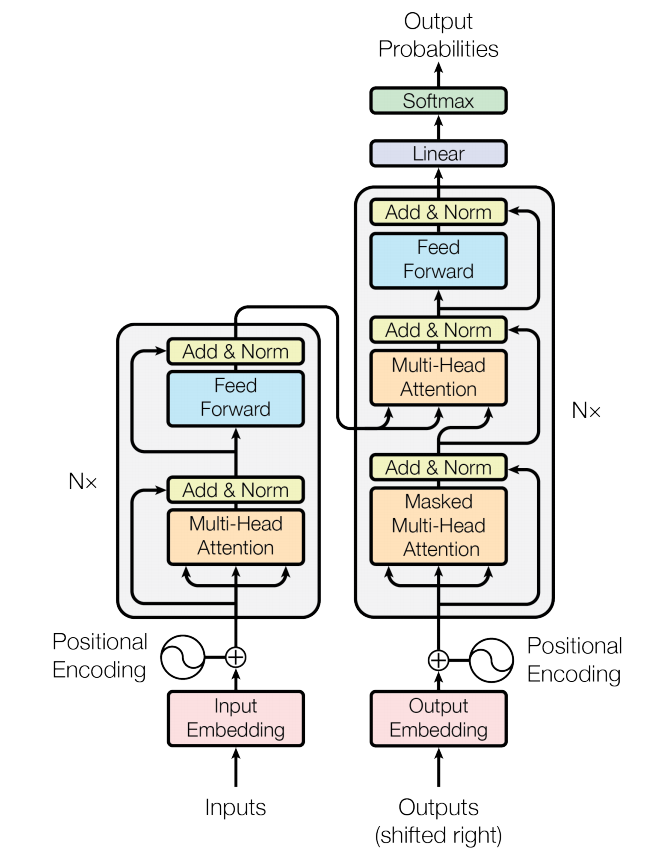
\includegraphics[width=0.95\linewidth]{imagenes/transformer-arquitectura.png} 
\caption{Arquitectura del \textit{transformer}.\\Fuente: \cite{NIPS2017_3f5ee243}}
\label{fig:arquitectura-transformer}
\end{wrapfigure}

\vspace{2mm}
En el \textbf{encoder} (parte izquierda de la \Cref{fig:arquitectura-transformer}), se encuentra un \textit{stack} de 6 capas. Cada una de estas, está compuesta por dos subcapas: una capa de \textit{Multi-Head Self-Attention} (un mecanismo de atención que se explicará más adelante); y una capa que contiene una red \textit{feed-forward} totalmente conectada. Cada una de estas subcapas, cuenta además con una conexión residual, que conecta la entrada de la subcapa con su salida de forma que puedan ser sumadas y normalizadas. Para facilitar la suma y normalización de entradas y salidas, todas las capas del modelo producen elementos de dimensión $d=512$. Antes de estas 6 capas, cada uno de los \textit{tokens} - elementos de la secuencia - de entrada (en la propuesta inicial, palabras), se convierten a vectores de dimensión $d$ a través de un \textit{embedding}\footnote{Operación que transforma, en el caso de la publicación original, palabras, en una representación numérica en un espacio vectorial donde las palabras con significado similar se encuentran próximas entre sí} previamente entrenado y se les añade una codificación posicional (en esta propuesta, generada a partir de funciones seno y coseno de distintas frecuencias) que aporta al modelo información sobre la posición de cada \textit{token} dentro de la secuencia inicial.

\vspace{2mm}
Por otro lado, en el \textbf{decoder} (parte derecha de la \Cref{fig:arquitectura-transformer}), se vuelve a encontrar un \textit{embedding} previamente entrenado que transforma las salidas del modelo desplazadas una posición. Al resultado de este \textit{embedding}, se le añade una codificación posicional similar a la del \textit{encoder}. A continuación, hay otro \textit{stack} de 6 capas, que esta vez está compuesto por las dos subcapas que están presentes en el \textit{encoder} (en este caso la capa de \textit{Multi-Head Self-Attention} es en realidad \textit{Multi-Head Masked Self-Attention} ya que se aplica una máscara para evitar que influyan en la red los \textit{tokens} siguientes al \textit{token} que se va a predecir), y una subcapa adicional de \textit{Multi-Head Cross-Attention}, situada entre las otras dos subcapas, donde las salidas de la subcapa de \textit{masked self-attention} del \textit{decoder} pueden acceder a las salidas del conjunto de capas del \textit{encoder}. (\textbf{La entrada de esta última capa de atención proviene de la última capa del \textit{encoder}, no de sus capas intermedias}). Por último, a la salida del \textit{stack} de capas del \textit{decoder}, se encuentra una transformación lineal (entrenada) y una función softmax para predecir la salida de la red.

% \paragraph{Mecanismos de atención}\mbox{}\\
\subsubsection{Mecanismos de atención}\label{bloques-atencion}

\vspace{2mm}
Los mecanismos de atención, presentados por primera vez en \cite{neuralmachinetranslationalignandtranslate}, buscan simular la atención cognitiva y han sido previamente empleados en redes recurrentes \cite{pmlr-v37-xuc15} y convolucionales \cite{7298685, 7410695} para aprender qué partes de la entrada son más relevantes en la tarea a completar. Sin embargo, en \cite{NIPS2017_3f5ee243}, con los \textit{transformers}, se propone por primera vez una arquitectura basada solamente en estos mecanismos. 

% \sout{De esta forma, se eliminan los sesgos cognitivos \cite{} que se han introducido en arquitecturas anteriores para facilitar su aprendizaje y mejorar su funcionamiento. Dichos sesgos cognitivos, son, por ejemplo, el uso de convoluciones para tratamiento de imágenes, donde se presupone que los elementos más cercanos a un píxel serán de mayor interés; o el uso de redes recurrentes secuenciales para procesamiento de lenguaje natural, donde se almacena toda la información que precede a un elemento de forma conjunta.} 
Las funciones de atención más empleadas son la atención aditiva \cite{neuralmachinetranslationalignandtranslate} y multiplicativa, siendo esta última la empleada en los \textit{transformers}, donde la atención se consigue a través de un producto escalar dentro de un bloque con múltiples cabezas llamado \textit{Multi-Head Attention}, elementos principales de los \textit{transformers}, que aparecen de dos formas distintas:
\begin{itemize}
    \item Bloques de \textit{Self-Attention}, en el \textit{encoder} y en el \textit{decoder}, con todas las entradas dentro de sus respectivas capas.
    \item Bloques de \textit{Cross-Attention}, en las capas del \textit{decoder}, con entradas provenientes del final de la pila de capas del \textit{encoder} y de la subcapa anterior del \textit{decoder}.
\end{itemize}
Cada una de las cabezas que componen estos bloques basan su funcionamiento en multiplicar sus entradas por una serie de matrices $W^V$, $W^K$ y $W^Q$ que son aprendidas durante el entrenamiento, de donde se obtienen, respectivamente, vectores \textit{Value} (V), \textit{Key} (K) y \textit{Query} (Q). Estos vectores, permiten que cada uno de los elementos de la secuencia de entrada, con el cálculo asociado a la atención (\Cref{fig:multi-head-attention}) soliciten a través de su vector \textit{Query} la información que determinen más importante de la secuencia. Esto se consigue al calcular el producto escalar de todos los vectores Q con todos los vectores K, que resultará mayor cuanto más alineados estén ambos vectores - mayor similitud entre las \textit{Queries} (consultas) y las \textit{Keys} (claves) -. A los resultados de estos productos escalares, se les aplica una función \textit{SoftMax} para asegurar que sumen una unidad y finalmente se multiplican por los vectores V para obtener el resultado final de la atención. Los resultados de todas las cabezas, se concatenan en una sola matriz para aprovechar al máximo el procesamiento en paralelo y atraviesan una última proyección linear.

Al usar solamente mecanismos de atención y cruzar toda la secuencia de entrada con sí misma, la longitud de esta deja de ser relevante, ya que cualquier elemento de la entrada puede obtener información de otro elemento, independientemente de lo alejado que esté (a diferencia de las redes recurrentes, donde la información de los elementos alejados perdía significado).

% \todo[inline]{En el anexo 1, hacer algo similar a \url{https://youtu.be/4Bdc55j80l8} + \url{https://jalammar.github.io/illustrated-transformer/}}

\begin{figure}[H]
\centering
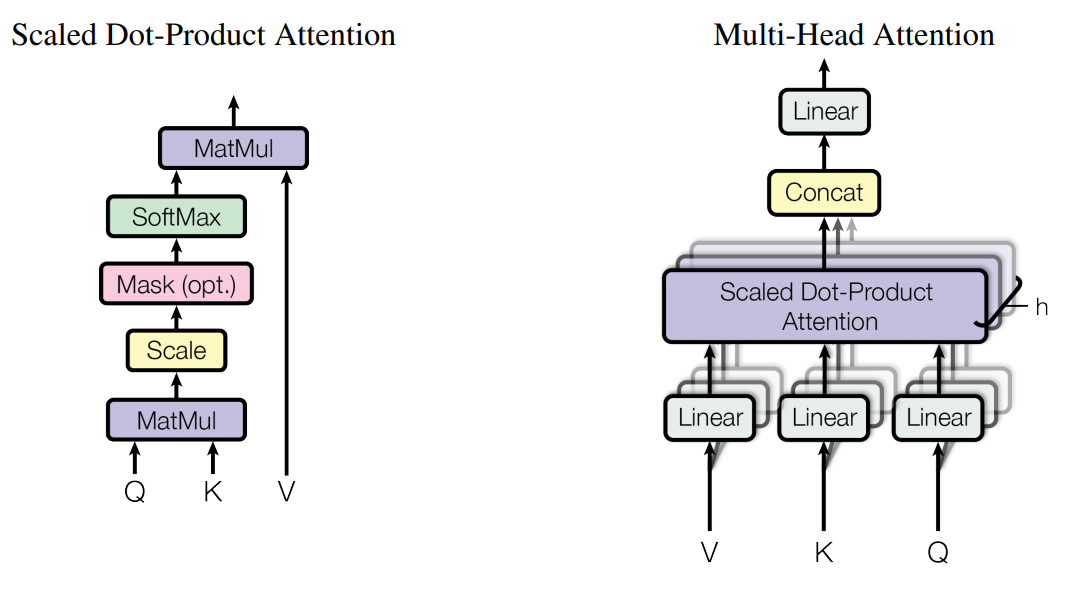
\includegraphics[width=0.65\linewidth]{imagenes/multi-head-attention.png} 
\captionsetup{width=.8\linewidth}
\caption{Producto escalar para el cálculo de la atención (izquierda) y bloque de \textit{Multi-Head Attention} (derecha). Fuente: \cite{NIPS2017_3f5ee243}}
\label{fig:multi-head-attention}
\end{figure}

No obstante, estos mecanismos de atención son considerablemente costosos, ya que tienen una complejidad $O(n^{2})$ tanto en tiempo como en memoria, siendo n el número de elementos de la secuencia de entrada (al bloque de atención). Es por esta razón por lo que han ido surgiendo una serie de propuestas para reducir dicha complejidad computacional, algunas de las cuales se exponen en la siguiente sección.



\subsubsection{Atención eficiente}\label[seccion]{atencion-eficiente}
% se puede seguir la línea de \cite{2020arXiv200906732T} pero quitando los modelos que no nos interesen y profundizando en los papers de los modelos que sí. Ver si hay papers especificos de pruning en transformers que cuenten algo interesante ; https://arxiv.org/abs/1910.14488

Para reducir los requisitos de memoria y el coste computacional de los \textit{transformers}, que tal y como se ha mencionado anteriormente, obtienen sus resultados gracias a los mecanismos de atención, pero que sin embargo son muy costosos computacionalmente, surgen distintas técnicas que buscan aproximar el resultado de la multiplicación de matrices que se lleva a cabo en los bloques de atención. Siguiendo el esquema propuesto en \cite{2020arXiv200906732T}, estas modificaciones de las capas de atención pueden agruparse en:

\paragraph{Patrones fijos - Fixed Patterns (FP)}:
En los patrones fijos, la longitud de la secuencia de entrada a los mecanismos de atención se reduce, por ejemplo: accediendo a ella en bloques de un tamaño determinado, en esto se basan \textbfit{Blockwise Attention} \cite{qiu-etal-2020-blockwise} y \textbfit{Local Attention} \cite{localattention}; accediendo a la secuencia en intervalos previamente definidos, como en \textbfit{Sparse Transformer} \cite{sparse-transformers} o \textbfit{Longformer} \cite{beltagy2020longformer} donde se emplean ventanas dilatadas o con un determinado \textit{stride} (zancada); o también empleando operaciones de \textit{pooling} para reducir la longitud de la entrada, en \textbfit{Compressed Attention} \cite{j.2018generating}.

\paragraph{Combinación de patrones - Combination of Patterns (CP)}:
Este grupo de métodos, se basa principalmente en la combinación de diferentes patrones de acceso a los elementos que componen la secuencia de entrada y aparece en \textbfit{Sparse Transformer} \cite{sparse-transformers} donde se combinan \textit{Local Attention} y \textit{strided attention} asignando la mitad de las cabezas del bloque de \textit{multi-head attention} a cada uno de los métodos. También aparece en \textbfit{Axial Transformer} \cite{ho2019axial}, donde la atención se aplica de forma independiente en cada uno de los ejes de la entrada (en este caso, el tensor de entrada debería ser multidimensional).

\paragraph{Aprendizaje de patrones - Learnable Patterns (LP)}:
Pese a ser similar a los dos casos anteriores ya que siguen basándose en diferentes formas de acceder a la secuencia de entrada para hacerla más dispersa, estos métodos son capaces de aprender en la etapa de entrenamiento del modelo qué patrones de acceso son más adecuados. Algunas de las propuestas que emplean este tipo de patrones son \textbfit{Reformer} \cite{Kitaev2020Reformer:}, que agrupa los elementos de la secuencia de entrada (\textit{tokens}) empleando una medida de similitud en grupos de elementos (para posteriormente aplicar el mecanismo de atención de forma independiente en cada grupo) o \textbfit{Routing Transformer} \cite{routingtransformer} que emplea k-medias para agrupar los \textit{tokens}, ambos modelos, reducen la complejidad a $O(n \log n)$. Dentro de estos modelos también destaca \textbfit{ResT} \cite{zhql2021ResT}, que está enfocado a imágenes y emplea convoluciones separables para reducir las dimensiones de las entradas al mecanismo de atención.

\paragraph{Disminución de rango}:
Este conjunto de arquitecturas, incluyen una proyección para conseguir una aproximación de la matriz resultante del cálculo de la atención, esta aproximación, pese a tener el mismo número de elementos (filas), obtiene una representación de los vectores menor (columnas), por lo que la dimensión de la matriz pasa de ser $n \times n$ a ser $n \times k$, con la consecuente disminución de coste computacional. El principal ejemplo de este tipo de arquitectura es \textbfit{Linformer}, \cite{wang2020linformer} que presenta una complejidad $O(n)$

%\paragraph{Kernels}:
%Por último, y aunque podrían entrar dentro del grupo de disminución de rango, existen enfoques que emplean kernelización en los mecanismos de atención para evitar el cálculo explicito de la matriz $n \times n$. Un ejemplo de este tipo de enfoques es el propuesto en \cite{kernel-transformer}, que de nuevo reduce la complejidad a $O(n)$.

% TODO: Ver si performer se puede mencionar también en el grupo de kernels y ya hilarlo en el parrafo donde se hable de el.

\subsubsection{Performer}
En este trabajo se estudia la influencia de un mecanismo de atención eficiente concreto para sustituir la atención estándar de DPT. Este mecanismo es el propuesto por Choromanski et al. en \textit{Rethinking Attention with Performers}\cite{performers}, que reduce la complejidad de la atención de $O(n^2)$ a $O(n)$.

Para conseguir esta reducción de la complejidad, el método modifica el orden de multiplicación de las matrices $Q$ (\textit{Queries}), $K$ (\textit{Keys}) y $V$ (\textit{Values}) del mecanismo de atención estándar. Siendo $n$ el número de \textit{tokens} de dimensión $d$ de la cadena de entrada, si en vez de multiplicar $(Q \times K^T) \times V$ se multiplica $Q \times (K^T \times V)$, las dimensiones multiplicadas serían $(n \times d) \times ((d \times n) \times (n \times d))$ en vez de $((n \times d) \times (d \times n)) \times (n \times d)$. Es decir, el número de operaciones en la multiplicación pasaría de ser $2 n^2 d$ (atención estándar) a ser $2 d^2 n$ (\textit{performer}), haciendo que el coste crezca de manera lineal con el número de \textit{tokens} si $n >>>> d$.

No obstante, hay un problema importante, y es que antes de multiplicar la matriz de atención ($Q \times K^T$) por la matriz $V$, se le aplica una función \textit{softmax} (\Cref{fig:multi-head-attention}) que al ser no lineal, impide la reasociación de la multiplicación de matrices. Para solucionar esto, los autores presentan un método basado en \textit{kernelización} y \textit{random Fourier features} que permite aproximar el resultado de aplicar la función \textit{softmax} a matriz de atención con dos matrices $Q'$ y $K'$ (de dimensiones $n \times r$) sin necesidad de calcular $Q \times K^T$ para así poder modificar el orden de las operaciones (\Cref{fig:performer}). 

\vspace{-3mm}

\begin{figure}[H]
\centering
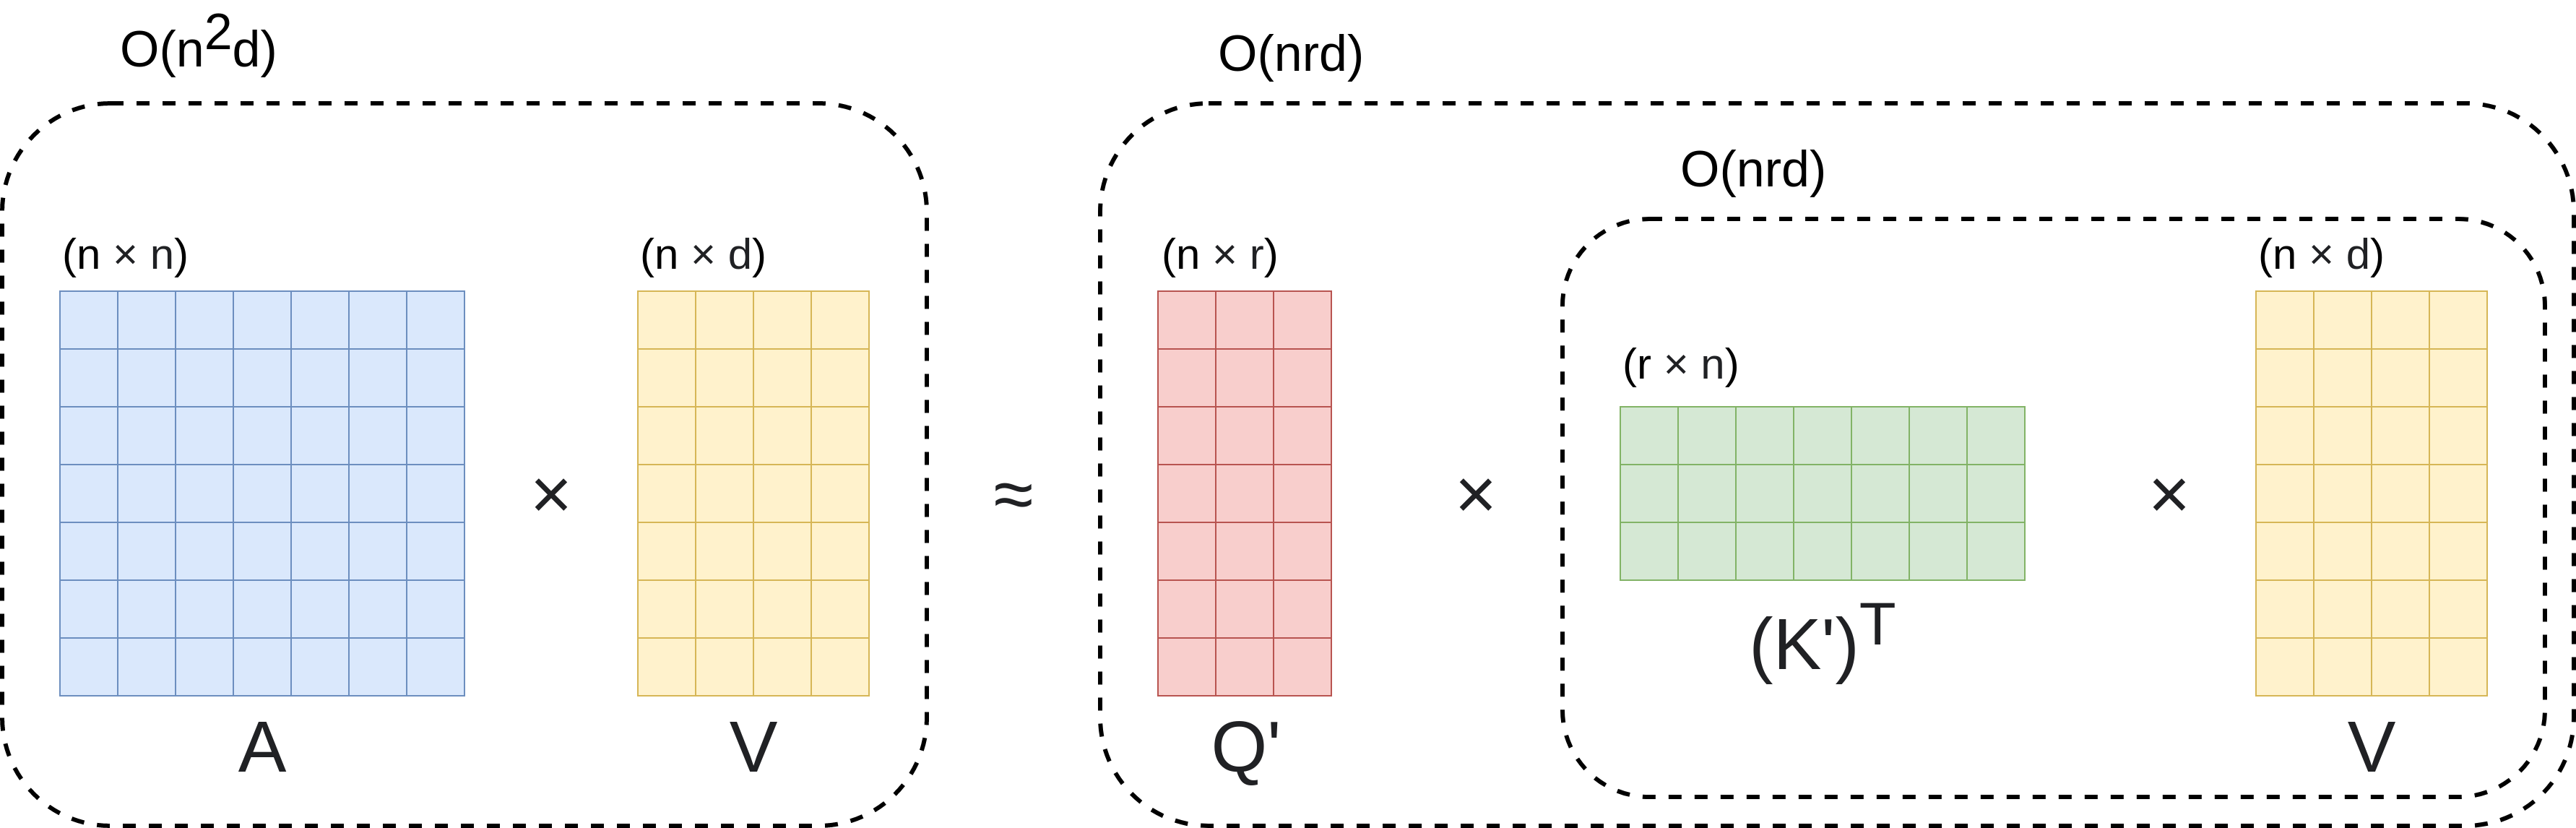
\includegraphics[width=1\linewidth]{imagenes/performer2.png} 
\captionsetup{width=1\linewidth}
\caption{Aproximación y reasociación del orden de multiplicación en el mecanismo de atención del \textit{Performer}. Figura inspirada en \cite{performers}.}
\label{fig:performer}
\end{figure}

% \todo[inline]{Video Kernels: \url{https://www.youtube.com/watch?v=y_RjsDHl5Y4}}
% \todo[inline]{Random Fourier Features}
% \todo[inline]{Video Performer: \url{https://www.youtube.com/watch?v=xJrKIPwVwGM&t=2s}}

\subsection{Transformers para visión artificial - ViT}
A la hora de aplicar la arquitectura de los \textit{transformers} a procesamiento de imágenes, surge un problema importante. La complejidad del mecanismo original de atención es $O(n^{2})$, siendo n el número de elementos en la secuencia de entrada, por lo que para una imagen de dimensiones $lado \times lado$, el número de píxeles que conformarían la secuencia de entrada al mecanismo de atención es $n = l^2$, disparando la complejidad de la atención a $O(l^{4})$. Para lidiar con este problema, se han propuesto distintas soluciones como limitar el mecanismo de atención al entorno de cada píxel (presentado en \textit{Image Transformers} \cite{image_transformer}) o aplicar convoluciones para reducir el tamaño de la secuencia de entrada \cite{detrfacebookdetectiontransformers}. 

Sin embargo, la solución propuesta en \textit{An Image is Worth 16x16 Words} con el \textit{Vision Transformer} \cite{image16x16words} es la que mejores resultados ha obtenido y por lo tanto aquella que más popularidad ha ganado como base de arquitecturas para otros problemas de visión artificial \cite{visiontransformersDPT, bhat2020adabins, chen2021transunet, liu2021Swin}. Esta solución, consiste en dividir la imagen original en fragmentos de tamaño fijo y convertir con una proyección cada fragmento en un vector de valores (\textit{embedding}). Estos vectores, son equivalentes al resultado del \textit{embedding} de palabras en la arquitectura original y se introducen al modelo como tal, es decir, cada fragmento extraído de la imagen correspondería a una palabra de una frase (\Cref{fig:vit}). Esta arquitectura, al ser inicialmente propuesta para realizar clasificación, solamente emplea el \textit{encoder} del \textit{transformer}.

\begin{figure}[H]
\centering
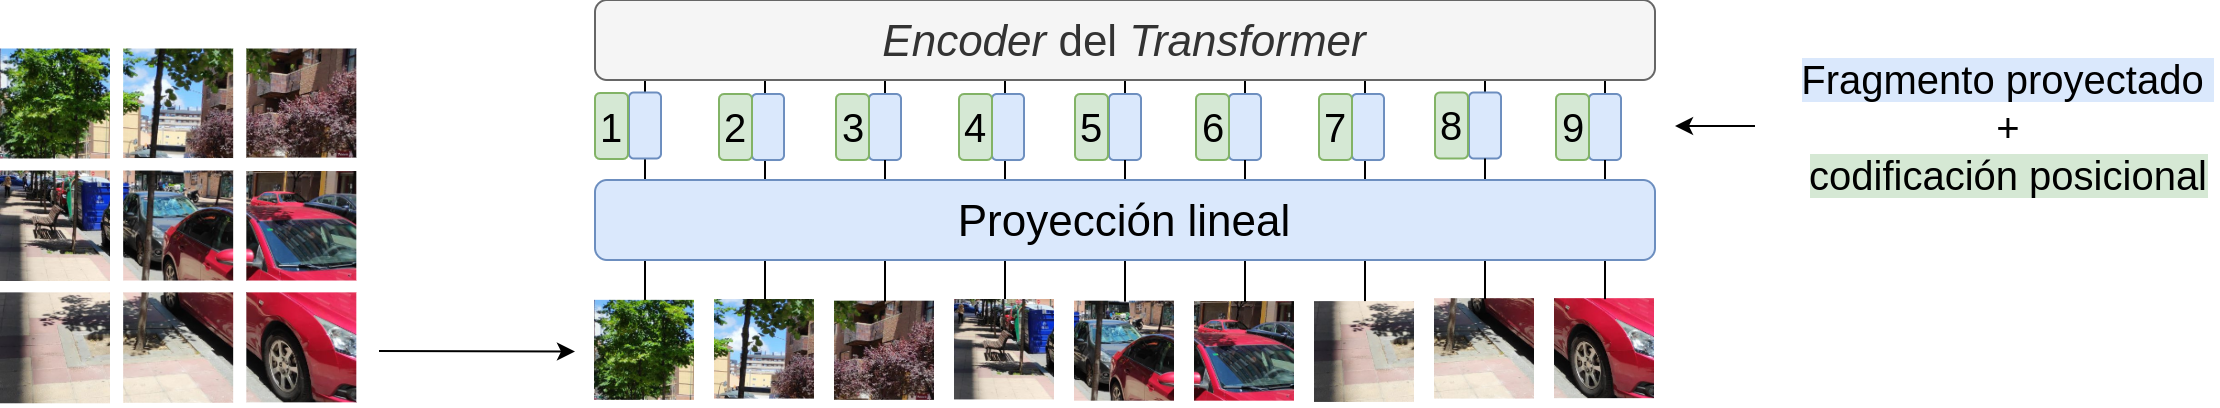
\includegraphics[width=1\linewidth]{imagenes/vit.png} 
\captionsetup{width=.8\linewidth}
\caption{\textit{Backbone} basado en fragmentos y proyección lineal del ViT. Figura inspirada en \cite{image16x16words}}
\label{fig:vit}
\end{figure}

En esta publicación, además, se presenta una variante del \textit{Vision Transformer}, el \textbfit{Hybrid Vision Transformer}. La diferencia entre esta arquitectura y la original es la sustitución del \textit{backbone} del ViT, es decir, de la separación en fragmentos y la proyección lineal, por una red convolucional de cuyos mapas de características se extraen los vectores que pasan a los bloques de atención (\Cref{fig:hybrid-vit}). Para formar estos vectores, en la implementación usada en este trabajo, se agrupan los mapas de características en función de sus píxeles, por lo tanto, si hay $n$ mapas de características, el píxel número 1 de cada uno de ellos formará un vector de dimensión n. De esta forma, la dimensión del vector viene dada por el número de mapas de características y el número de \textit{tokens} será equivalente al número de píxeles de los mapas de características (imágenes mayores conllevan un mayor número de \textit{tokens}).

\begin{figure}[H]
\centering
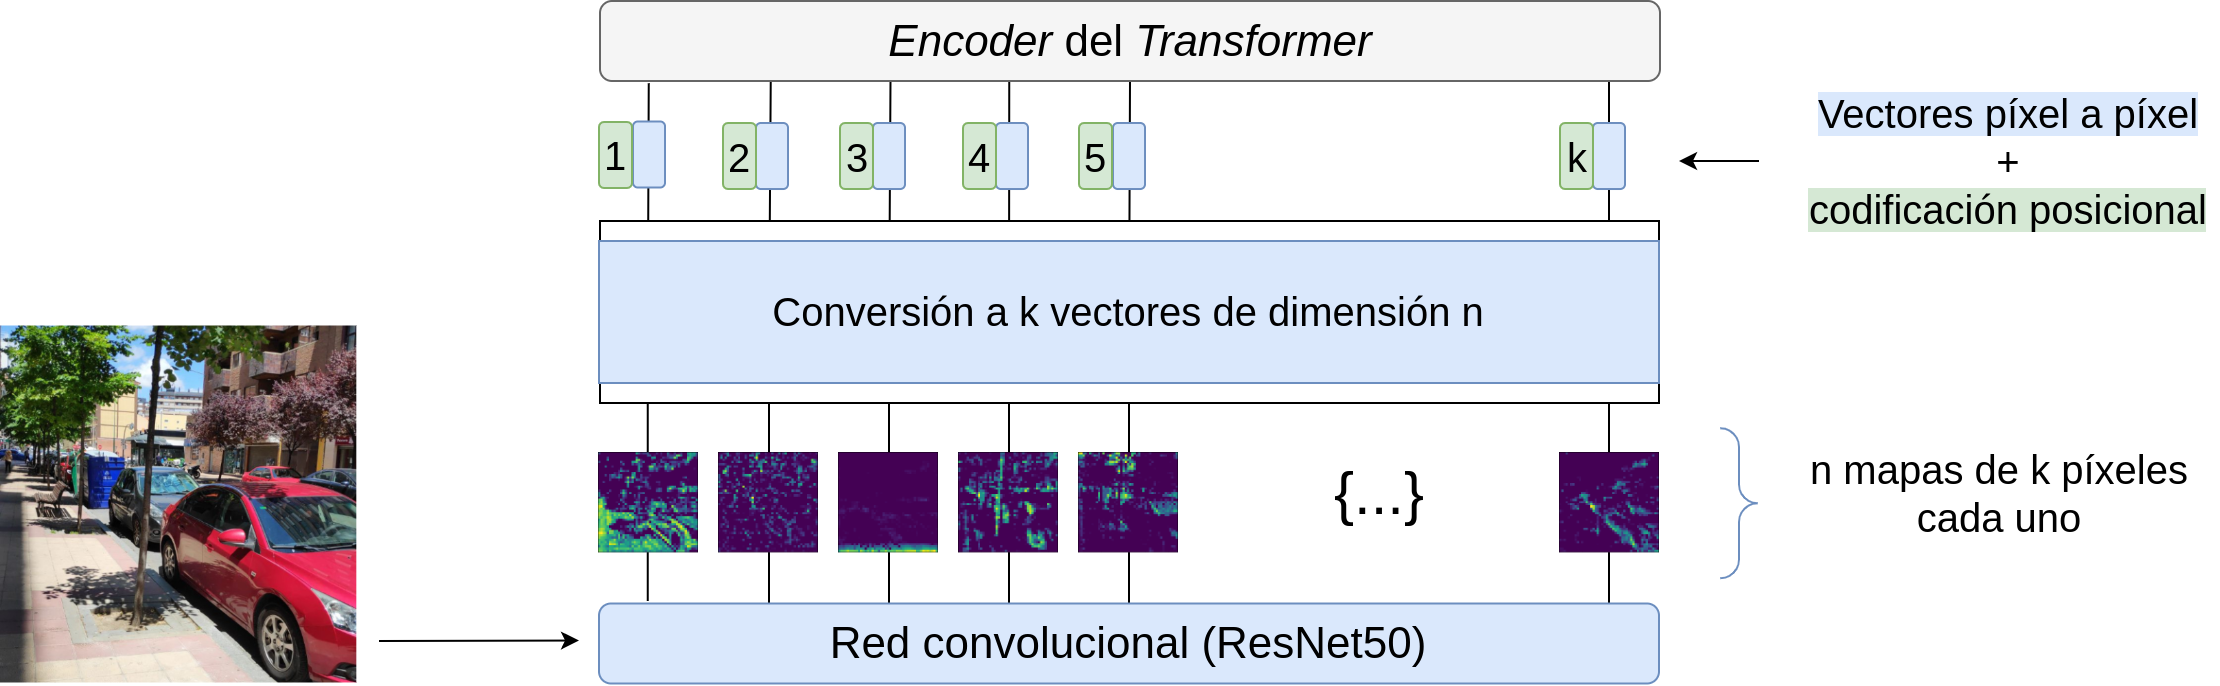
\includegraphics[width=1\linewidth]{imagenes/vit-hybrid.png} 
\captionsetup{width=.8\linewidth}
\caption{\textit{Backbone} convolucional del ViT-Hybrid.}
\label{fig:hybrid-vit}
\end{figure}

\subsection{Estimación de profundidades}
Otra de las bases fundamentales de este trabajo es la estimación de profundidades. Esta tarea, tanto cuando es llevada a cabo por humanos como por máquinas, consiste en detectar la distancia relativa entre todo aquello que se ve. Tal y como se ha mencionado en el capítulo de Introducción, el cerebro humano se apoya principalmente en la disparidad existente entra las imágenes que capturan cada uno de los ojos (estereovisión), ya que las cosas que están más lejanas ven su posición menos alterada entre la vista de un ojo y de otro que las cosas cercanas. Sin embargo, también capaz de estimar la profundidad en una sola imagen a partir de nuestro conocimiento previo del mundo y del entorno (pistas monoculares). 

Las técnicas de visión artificial tradicional (basadas en dos cámaras - visión estereoscópica) no pueden lidiar con este problema, por lo que la estimación monocular (con una sola cámara) es prácticamente imposible empleando técnicas tradicionales. Para este tipo de estimación (monocular), entran en juego los modelos de aprendizaje automático, que han demostrado una gran capacidad para explotar el conocimiento sobre el entorno en todo tipo de tareas, no siendo la estimación de profundidades diferente. 

A continuación, aunque haciendo especial hincapié en aquellos basados en aprendizaje automático, se enumeran los distintos enfoques existentes, incluyendo aquellos propios de la visión artificial tradicional, las soluciones \textit{hardware}, y las técnicas de aprendizaje profundo.

\subsubsection{Técnicas de estimación de profundidades} \label[seccion]{estimacion-profundidades-sota}

La estimación de profundidades se ha intentado resolver de múltiples maneras \cite{Zhao_2020}. Dentro de estas metodologías, existen tres enfoques principales en función del tipo de \textit{software} o \textit{hardware} que se emplea.
\begin{itemize}
    \item \textbf{Soluciones geométricas}: Este grupo de métodos extrae información de las restricciones geométricas que existen entre parejas de imágenes. Principalmente se agrupan en técnicas de \textit{SfM (Structure from Motion}) donde se reconstruye la tercera dimensión a partir de imágenes tomadas por una sola cámara en movimiento, y en técnicas de estereovisión, donde la profundidad se obtiene de la disparidad entre las imágenes capturadas por una pareja de cámaras con posiciones relativas conocidas. Estos métodos, sin embargo, basan su funcionamiento en el emparejamiento de puntos claves (\textit{feature points}) que deben encontrarse en ambas imágenes, requiriendo por lo tanto texturas o formas características que poder emparejar.
    \item \textbf{Soluciones hardware}: Por otro lado, existen una serie de soluciones basadas en distintos sensores como son los LIDAR, las cámaras de tiempo de vuelo (ToF) o los escáneres de luz estructurada. Estas soluciones, no obstante, cuentan con ciertas limitaciones como son la densidad de sus capturas (representaciones de puntos dispersos en el caso del LIDAR\footnote{Por representaciones dispersas se entiende la captura de la profundidad en forma de una nube de puntos discretos separados entre sí, mientras que una representación densa tiene una mayor cantidad de puntos de información.}), la sensibilidad a la iluminación (en las cámaras ToF) o su rango de acción y la necesidad de un entorno controlado (luz estructurada).
    \item \textbf{Aprendizaje automático}: Debido a las restricciones de los métodos existentes y a los resultados obtenidos empleando aprendizaje automático en otros campos de la visión artificial, en los últimos años han surgido múltiples arquitecturas enfocadas a recuperar la profundidad a partir de imágenes. Este documento, pese a revisar superficialmente otras opciones, se centra en las \textbf{soluciones monoculares} debido al interés detrás de obtener una representación de la profundidad a partir de una sola cámara (coste, espacio, consumo, etc.).
\end{itemize}

% Buen resumen para estirar -> \url{https://towardsdatascience.com/depth-estimation-1-basics-and-intuition-86f2c9538cd1}}

% https://openaccess.thecvf.com/content_CVPR_2020/papers/Johnston_Self-Supervised_Monocular_Trained_Depth_Estimation_Using_Self-Attention_and_Discrete_Disparity_CVPR_2020_paper.pdf

\subsubsection{Aprendizaje automático no supervisado}

Estas propuestas, ofrecen soluciones que emplean datos sin etiquetar debido a la dificultad que entraña la obtención de este tipo de anotaciones. Normalmente, estas soluciones emplean secuencias (vídeos) de imágenes monoculares, extrayendo automáticamente a partir de estas una señal supervisora con distintos métodos. En \cite{zhou2017unsupervised} se propone una arquitectura que emplea una red neuronal para calcular la posición (y movimiento) de la cámara entre \textit{frames} consecutivos (\textit{ego-motion}), que a su vez se emplea para calcular la profundidad de la imagen. Sin embargo, da por hecho que ningún objeto ha cambiado de posición y que el entorno es estático. 

Esto, no es aplicable a entornos reales, por lo que surgen diferentes arquitecturas que generan máscaras, tanto basadas en redes neuronales \cite{zhou2017unsupervised, vijayanarasimhan2017sfmnet} como en técnicas geométricas \cite{geo_mask_egomotion, monodepth}, para lidiar con los objetos dinámicos. Otros enfoques, con la misma idea subyacente, sustituyen la red de estimación de posición con métodos de odometría visual\footnote{La odometría agrupa aquellas técnicas que estiman el cambio de posición a partir de las lecturas de sensores. En el caso de la odometría visual, estos cambios de posición se estiman empleando principalmente imágenes capturadas por una cámara.} tradicional \cite{visualodometryunsupervised}, que puede aportar posiciones más exactas y mejorar el funcionamiento final. Por último, algunos enfoques calculan elementos adicionales como por ejemplo el flujo óptico de la escena (cálculo de los patrones de movimiento para cada punto de la imagen) que aporta información relevante sobre la posición relativa de los objetos \cite{vijayanarasimhan2017sfmnet, geonet}. 

\subsubsection{Aprendizaje automático semisupervisado}

Debido también a la escasez de datos etiquetados, también son populares los enfoques semi supervisados. Estas soluciones, emplean información parcial como señal supervisora, que complementan con información no etiquetada. Algunos ejemplos característicos de este tipo de aprendizaje son: 
\begin{itemize}
    \item Síntesis artificial de parejas a partir de imágenes monoculares para emplear técnicas de estereovisión, entrenando los modelos con parejas de imágenes obtenidas por conjuntos de cámaras preparados para estéreo \cite{monocularstereosynthesis, single-view-stereo-matching}.
    \item Generación de los mapas de disparidad entre parejas de imágenes para estereovisión \cite{importancestereo, deep3d}, donde la señal supervisora es la disparidad obtenida mediante técnicas tradicionales de estereovisión.
    \item Utilización de datos etiquetados de forma dispersa (frecuentemente obtenidos con dispositivos LIDAR), que o bien emplean imágenes no etiquetadas para densificar dichas representaciones \cite{lidarcompletion, sparse-to-dense, hu2020PENet} o añaden la información del LIDAR en la función de perdidas para después inferir a partir de imagen monocular \cite{lidarlossfunction}.
\end{itemize}

\subsubsection{Aprendizaje automático supervisado} \label[seccion]{aprendizaje-supervisado}
% Ver CRFs en condiciones
Pese a la dificultad para obtener datos etiquetados correctamente, los enfoques supervisados siguen siendo los que mejores resultados ofrecen y por lo tanto han sido y siguen siendo extensamente estudiados. El primero de estos modelos fue propuesto en \cite{eigen-multi-scale}, y empleaba dos conjuntos de capas, uno para generar una estimación tosca de la profundidad y otro para refinar esa primera estimación. Enfoques posteriores propusieron modificaciones en la función de perdidas para fomentar la consistencia en las predicciones \cite{surfacenormals} a través del cálculo de los gradientes de la diferencia entre el resultado y el objetivo. Además de aquellos basados en arquitecturas \textit{encoder-decoder}, también hay propuestas con arquitecturas de aprendizaje adversario \cite{gan} donde el discriminador trata de distinguir entre la profundidad generada y la real \cite{gan-depth}.

% DPT ajusta mínimos cuadrados la predicción con el ground truth para sacar un factor de escala, AdaBins da profundidades en metros.
Todas estas soluciones, basan su funcionamiento en redes convolucionales, sin embargo, los \textit{transformers} han presentado muy buenos resultados en los últimos años y también se han propuesto soluciones que emplean estas arquitecturas, en el momento de redactar este documento, predominan dos: los \textbfit{Dense Prediction Transformers} (DPT) \cite{visiontransformersDPT} y \textbfit{AdaBins} \cite{bhat2020adabins}.

El primero de estos dos modelos, al ser la arquitectura que se modifica a lo largo del proyecto, se explica en mayor profundidad en la siguiente sección. El segundo, \textit{AdaBins}, está compuesto de un \textit{encoder} convolucional y una etapa inspirada en los \textit{Vision Transformers} \cite{image16x16words} que recibe la salida de el \textit{encoder} y clasifica cada píxel en un histograma de profundidades cuyas barras (\textit{bins}) son parametrizadas (centro y rango) dinámicamente para cada imagen. El resultado final se consigue con la suma ponderada de la predicción de pertenencia a cada barra y el valor medio de dicha barra, consiguiendo así una estimación de profundidad suavizada.


\subsubsection{DPT}\label[seccion]{DPT}
Tal y como se ha mencionado previamente, la gran mayoría de arquitecturas de estimación de profundidades se basan en redes convolucionales, normalmente de tipo \textit{encoder-decoder}. Las líneas de investigación se centran en el \textit{decoder} y sus estrategias de agregación de información. DPT (\textit{Dense Prediction Transformer}) \cite{visiontransformersDPT} también se estructura como un \textit{encoder-decoder}, pero centra su estudio en la modificación del \textit{encoder} debido a la gran influencia que tiene este en la información que llega a la segunda parte de la red, sustituyendolo por una arquitectura basada en mecanismos de atención (\textit{transformer}). De esta forma, gracias a las características propias de estos modelos ya comentadas, la arquitectura se beneficia de un campo receptivo que permite atender a la información de toda la imagen en las etapas de atención. Es decir, se pasa de un campo receptivo local mucho más limitado (en las redes convolucionales) a un campo receptivo global.

\begin{figure}[H]
\centering
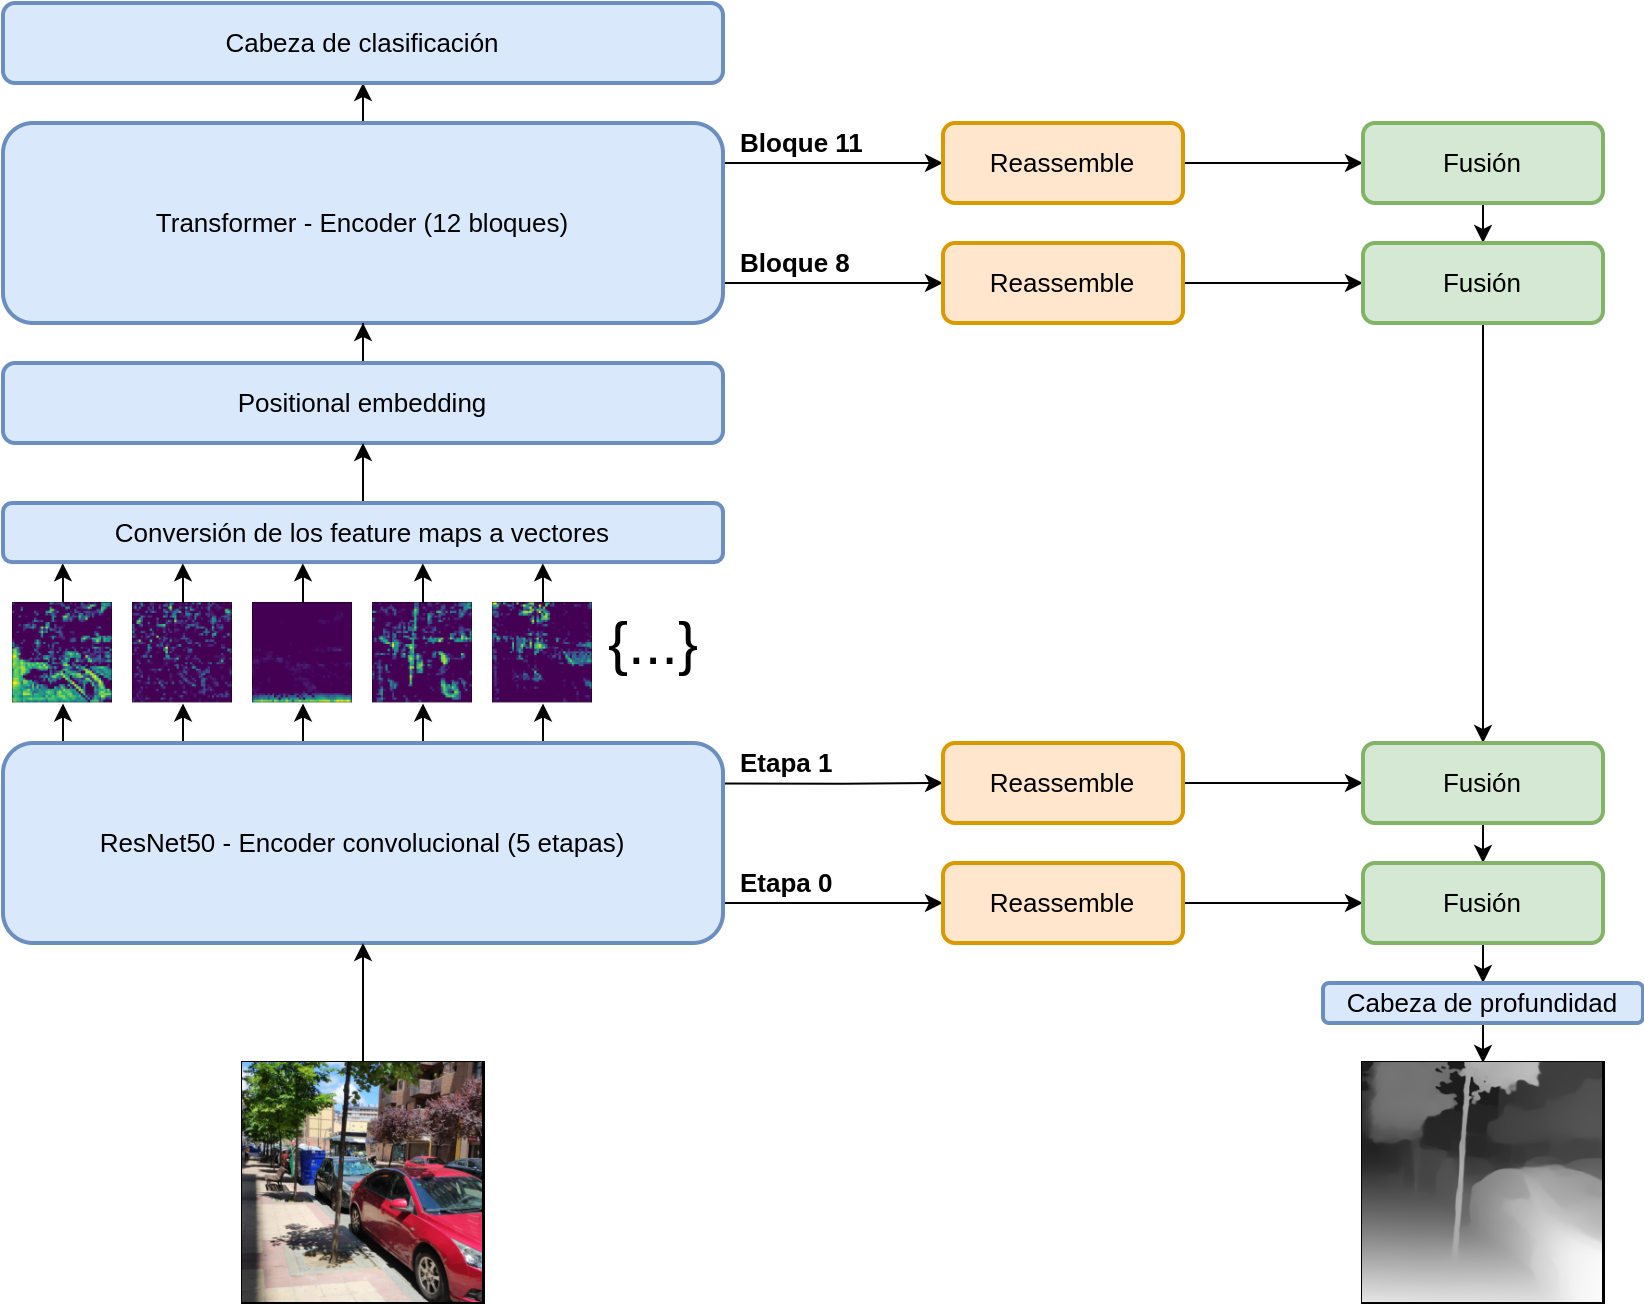
\includegraphics[width=\linewidth]{imagenes/DPT-general.png} 
\captionsetup{width=.7\linewidth}
\caption{Esquema de la arquitectura de DPT-Hybrid.}
\label{fig:dpt-hybrid}
\end{figure}

En la publicación que presenta este modelo se utilizan tres variantes del \textit{Vision Transformer} como \textbfit{encoder} para llevar a cabo los experimentos: ViT-Base, con \textit{embedding} de las imágenes a partir de fragmentos y $12$ bloques de atención; ViT-Large, con el mismo método de \textit{embedding} (esta vez con vectores de mayor dimensión para representar cada uno de los fragmentos codificados) y $24$ bloques de atención, y por último, ViT-Hybrid, con el mecanismo de \textit{embedding} de las entradas basados en una red convolucional (ResNet50) tal como se indica en la \Cref{fig:dpt-hybrid} seguido de $12$ bloques de atención.

Por otro lado, el \textbfit{decoder} de la arquitectura está compuesto por una serie de capas convolucionales que transforman representaciones extraídas de distintas etapas del \textit{encoder}. En el caso del ViT-Base, las representaciones a la salida de los bloques de atención $\{3, 6, 9, 12\}$, del ViT-Large, las correspondientes a las salidas de los bloques de atención $\{5, 12, 18, 24\}$, por último, en el caso del ViT-Hybrid, son las representaciones obtenidas de los bloques de atención $\{9, 12\}$ junto con las representaciones a la salida de la primera y segunda etapa de la ResNet50 encargada del \textit{embedding}.

Estas representaciones, como están en forma de \textit{tokens} en el caso de los bloques de atención, o en forma de mapas de características cuando se extraen de la ResNet50, atraviesan un bloque \textit{Reassemble} donde la información se concatena para reconstruir la estructura de imagen (\Cref{fig:reassemble-fusion}), se proyecta en el número de canales deseado, y se escala a una resolución determinada en función de la altura del \textit{encoder} de la cual provienen (cuanto antes se extraen las características, menos se reduce su tamaño, haciendo una especie de pirámide de resolución).

Una vez se dispone de los datos en un formato similar a imágenes (a la salida de los bloques de \textit{Reassemble}), pasan a una etapa similar a la arquitectura RefineNet \cite{refinenet}, que duplica el tamaño de cada una de las representaciones y las suma de forma escalonada (\Cref{fig:reassemble-fusion} y \Cref{fig:dpt-hybrid}) para fusionar su información.

\begin{figure}[H]
\centering
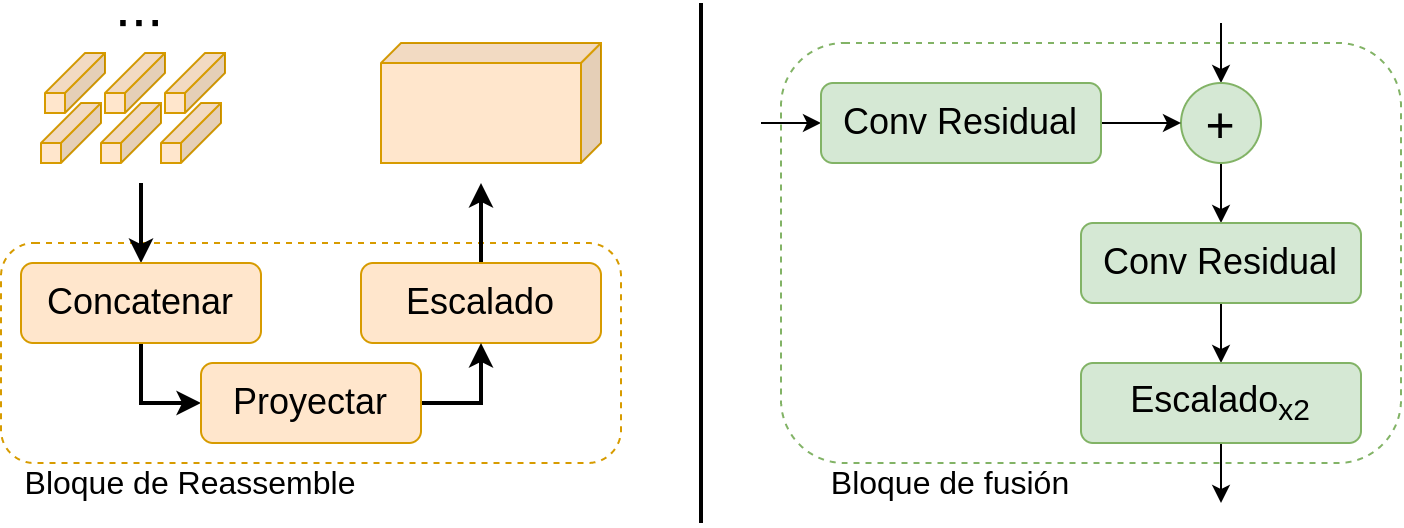
\includegraphics[width=0.7\linewidth]{imagenes/reassemble-fusion.png} 
\captionsetup{width=.7\linewidth}
\caption{Bloques base del \textit{decoder} de DPT. Izquierda: Bloque de \textit{Reassemble}. Derecha: Bloque de fusión. Figura adaptada de \cite{visiontransformersDPT}.}
\label{fig:reassemble-fusion}
\end{figure}

El resultado de este último bloque (una imagen con la mitad de la resolución de la entrada), pasa a una última etapa (cabeza especializada\footnote{En la publicación original, se adapta la red para segmentación semántica y para estimación de profundidades monocular. Dado que escapa del alcance de este proyecto, no se discuten en este documento las capacidades de DPT para segmentar objetos.}) para proporcionar la predicción final.

Antes de pasar a la metodología empleada en el trabajo original de DPT para entrenar los modelos, cabe mencionar que la red, tal y como se comenta a continuación, se entrena con una función de pérdida invariante a la escala y al desplazamiento. Esto significa que la profundidad obtenida del modelo es relativa y no un valor métrico medible. No obstante, los autores extraen valores de desviación y escala (ajustando por mínimos cuadrados las predicciones y las anotaciones en el conjunto de entrenamiento) con los que es posible transformar las profundidades relativas obtenidas en entradas nuevas a profundidades métricas (siempre y cuando la naturaleza de las entradas sea la misma que la de los ejemplos utilizados para obtener los valores de desplazamiento y escala).

\textbf{Entrenamiento}
% https://github.com/isl-org/DPT/issues/3#issuecomment-839883934
Los modelos proporcionados junto a la publicación, y en concreto, el que se emplea como base de este trabajo, fueron preentrenados en MIX6 (\Cref{mix6}) y después ajustados a otros \textit{datasets} para su evaluación. El entrenamiento en MIX6 se lleva a cabo empleando Adam como optimizador con un \textit{learning rate} de $1e-5$ para el \textit{encoder} y de $1e-4$ para el \textit{decoder} y se parte de parámetros preentrenados en Imagenet (\textit{encoder}) y inicializados aleatoriamente (\textit{decoder}). En cuanto a la duración del entrenamiento, el modelo se entrena durante 60 épocas, cada una con 72000 pasos y un \textit{batch size} de 16 imágenes. Además, se voltean horizontalmente las imágenes de manera aleatoria como forma de \textit{data augmentation}. Como función de coste, se utiliza una función de pérdida \cite{midas-intel} invariante a la escala (relativa) y al desplazamiento de la salida junto a otra función de pérdida que compara los gradientes\footnote{A la hora de entrenar en otros \textit{datasets}, desactivan esta función de pérdida si la anotación no es profundidad densa, es decir, si hay píxeles sin anotar como ocurre por ejemplo en KITTI.} \cite{MegaDepthLi18} en los valores de profundidad de la salida y la anotación.

\subsection{Optimización de modelos}\label[seccion]{optimizacion-modelos}
% \todo[inline]{https://heartbeat.fritz.ai/the-5-algorithms-for-efficient-deep-learning-inference-on-small-devices-bcc2d18aa806}

% \todo[inline]{Hablar de las formas no especificas con las que se pueden acelerar las redes neuronales, sería mencionar las de la presentación de la quinta reunión hablando un poco de cada una de ellas. También se podría meter un pequeño apartado de hardware hablando de TPUs y FPGAs, habría que ver como se cuadra y como encaja con el resto del apartado. Esto puede que para el TFM haya que recortarlo un poco también de cara a acotar un poco el estudio si no se va a hacer nada de esto (centrarnos en velocidad sin entrar en restricciones de memoria, por ejemplo)}
% \paragraph{Basadas en Hardware}\mbox{}\\
% \todo[inline]{Mencionar que hay TPUs (ASICs), GPUs, ... A lo mejor es conveniente sacar esto a un apartado de aceleración por hardware distinto de los mecanismo de eficiencia. La clasificación que hacen en las diapositivas de la clase de Stanford está bastante bien, se puede hablar de las cuatro cosas centrandonos en software para inferencia. ; \url{https://youtu.be/eZdOkDtYMoo} ; \url{http://cs231n.stanford.edu/slides/2017/cs231n_2017_lecture15.pdf}}

% \paragraph{Basadas en Software}\mbox{}\\
Los modelos de aprendizaje automático del estado del arte tienden a ser cada vez más grandes. Esto generalmente conlleva un tiempo de entrenamiento y de inferencia mayor, así como unos requisitos de memoria y consumos de energía mayores. Para solucionar algunos de los problemas asociados, como por ejemplo la necesidad de proporcionar buenos resultados con restricciones temporales o restricciones de \textit{hardware} (modelos embebidos, dispositivos móviles, etc.) han ido surgiendo a lo largo de los años una serie de soluciones que tratan estos aspectos, buscando siempre perjudicar lo mínimo posible los resultados de los modelos originales. A continuación, se presentan algunas de las más generales, aplicables en una gran variedad de arquitecturas.
% \todo[inline]{Hablar de las que son aplicables a más de un tipo de red, si encontramos alguna que sea solo para convolucionales, por ejemplo, podemos mencionarlas todas de corrido diciendo que existen también técnicas que son aplicables a arquitecturas concretas pero que dado que nos vamos a centrar en los transformers no se entra en esto.}

% \todo{Ver en el correo de gmail de papers tfm practicas el deep compression}

\todo[inline]{Aquí puede que se profundice demasiado en algunos temas (poda, por ejemplo)}

\begin{itemize}
    \item \textbf{Poda / Pruning}: Consiste en eliminar de los modelos aquellas conexiones o neuronas que son redundantes o menos relevantes para la red, con el objetivo principal de reducir el tamaño del modelo, ya que las redes neuronales suelen estar sobredimensionas y son redundantes. Al reducir el tamaño del modelo, aumentar la velocidad con la que se realiza la inferencia\footnote{Dependiendo de las técnicas utilizadas para llevar a cabo la poda, pueden aparecer limitaciones en el hardware de uso general para trabajar con matrices dispersas, pero existen soluciones tanto hardware como software para trabajar con estos datos.} sin sacrificar la exactitud del modelo en exceso. Siguiendo la clasificación presentada en \cite{vadera2020methods}, los métodos más empleados de poda se pueden agrupar en dos grandes grupos: Basados en magnitud y basados en sensibilidad.
    \begin{itemize}
        \item \textbf{Métodos basados en magnitud}:  Estas técnicas, eliminan los parámetros basándose en su valor o en la influencia que tienen en la siguiente capa. Por ejemplo, un peso con un valor muy próximo a cero apenas influirá en la capa siguiente, y por lo tanto puede eliminarse. Estas técnicas, suelen llevarse a cabo eliminando parámetros y reentrenando la red de forma iterativa, repitiendo este proceso hasta encontrar un equilibrio entre reducción de tamaño y pérdida de exactitud. Han et al. \cite{NIPS2015_ae0eb3ee} presentaron, empleando este entrenamiento recursivo, resultados donde se eliminan más de un 90\% de los parámetros aumentando solamente en unas décimas el porcentaje de error en comparación con los modelos sin podar. 
        % En este trabajo, también se probaron dos puntos importantes: la regularización L1 proporciona mejores resultados antes del reentrenamiento, pero sin embargo la regularización L2 genera mejores resultados después de el reentrenamiento; y que estos entrenamientos sucesivos del modelo (siempre con un \textit{learning rate} menor que en el entrenamiento inicial), convergen en mejores valores para los pesos que han permanecido sin podar si se parte de los resultados del primer entrenamiento y no se reinicializan aleatoriamente
        Además de la poda de conexiones y neuronas, existen también distintas técnicas destinadas a podar con una menor granularidad, por ejemplo, mapas de características y filtros. Algunas de estas técnicas incluyen las basadas en la varianza entre canales \cite{7303876} o en el número medio de ceros que tienen los mapas de características \cite{2016arXiv160703250H} entre otras.
        
        \item \textbf{Métodos basados en sensibilidad}: Estos métodos, a diferencia de los basados en magnitud, buscan analizar el efecto de la modificación de los pesos en la función de perdida. Para ello, suelen centrarse en aproximar los cambios en la función de perdida a través de una serie de Taylor. Esta serie de Tylor, incluye una matriz hessiana, que se obtiene a partir de las segundas derivadas de la perdida respecto de los pesos. 
        Dado que el cálculo de la matriz hessiana es computacionalmente costoso, Lecun et al. en \textit{Optimal Brain Damage (OBD)} \cite{NIPS1989_6c9882bb} ignora los elementos que no están situados en la diagonal de la matriz, reduciendo la complejidad del cálculo considerablemente. Posteriormente, Hassibi et al. plantearon no descartar dichos valores en \textit{Optimal Brain Surgeon (OBS)} \cite{NIPS1993_b056eb15} pero sus cálculos son prohibitivos con el número de parámetros de las arquitecturas actuales. Estas series de Taylor, también se han empleado para la poda de canales y mapas de características en redes convolucionales, tanto con aproximaciones de primer orden \cite{molchanov2017pruning} como de segundo orden \cite{pmlr-v97-wang19g}. 
    \end{itemize}
    \item \textbf{Quantization}: La cuantificación tiene como objetivo convertir los parámetros de las redes almacenados en 32 bits en representaciones más pequeñas como son los números enteros (normalmente en 8 bits). Esta transformación, conlleva una perdida de calidad en los resultados de los modelos, pero reduce sus requisitos de memoria y acelera la inferencia de resultados. Esta aceleración viene dada por la velocidad a la que se pueden realizar operaciones con números enteros comparado con las operaciones con números en coma flotante. Existen principalmente tres tipos de cuantificación, dinámica, estática (estas dos se aplican sobre un modelo ya entrenado) y durante el entrenamiento (\textit{Quantization Aware Training}).
    \begin{itemize}
        \item \textbf{Cuantificación dinámica}: En este caso, no solo se convierten los pesos del modelo ya entrenado a enteros, sino que también se transforman las activaciones buscando los parámetros de dichas conversiones de forma dinámica durante la inferencia. Este tipo de cuantificación no requiere de datos pero sin embargo no es tan rápida como las otras dos al tener que realizar las transformaciones durante la inferencia.
        \item \textbf{Cuantificación estática}: De forma similar al caso dinámico, las activaciones de las capas se cuantifican durante la inferencia, sin embargo, en este caso una vez se ha entrenado la red se le pasan bloques adicionales de datos con los que se estiman los parámetros de estos procesos de cuantificación para acelerar la inferencia cuando se haya desplegado el modelo. De esta forma, pese a que es necesario tener datos adicionales (no hace falta que estén etiquetados), se alcanza una mayor velocidad de inferencia.
        \item \textbfit{Quantization Aware Training}: Por último, esta opción tiene en cuenta la cuantificación durante todo el proceso de entrenamiento simulando el efecto de la cuantificación en los pesos y activaciones de forma que influyan en la función de perdidas (las operaciones durante el entrenamiento siguen haciéndose en coma flotante). Este método, debido a la consideración de la cuantificación durante el entrenamiento, resulta en una inferencia más rápida y resultados superiores a los de los métodos anteriores. Sin embargo, no siempre es aplicable al requerir el entrenamiento del modelo.
    \end{itemize}
    % \todo[inline]{Esto se puede mirar en las referencias que hace Method for Pruning Deep Neural Networks al principio de la página 3 ; https://leimao.github.io/article/Neural-Networks-Quantization/}
    \item \textbfit{Weight clustering}: El \textit{clustering} de pesos, o \textit{weight sharing}, agrupa los pesos del modelo en un número determinado de \textit{clusters} para asignar a cada peso el valor del centroide de su grupo correspondiente. De esta forma, se reducen los requisitos de memoria del modelo, ya que solamente es necesario almacenar los índices que apuntan al vector de centroides, que al ser números enteros se pueden representar con un número de bits mucho menor (por ejemplo, en 8 bits, reduciendo el tamaño de la matriz de pesos original (cada uno 32 bits) a un cuarto de su tamaño).
    
    \item \textbf{Mixed-precision training}: Propuesto por primera vez en \cite{micikevicius2018mixed}, el entrenamiento con precisión mixta almacena los pesos, activaciones y gradientes en formato de coma flotante de media precisión (16bits - IEEE 754) en vez de simple precisión (32 bits). De esta forma, sin perder precisión, se reducen a cerca de la mitad los requisitos de memoria en el entrenamiento, que además se ve acelerado en las últimas arquitecturas de GPUs. 
    Para conseguirlo se llevan a cabo tres estrategias: Mantener una copia maestra de los pesos almacenada en FP32, escalar el resultado de la función de perdida y acumular ciertos resultados en FP32.
    \begin{enumerate}
    \item \textbf{Copia maestra de los pesos en FP32}: A pesar de que en el \textit{forward} y \textit{backward pass} del entrenamiento se usan valores FP16, se debe almacenar una copia maestra en FP32 de los pesos, que son los empleados en el optimizador para multiplicar por gradientes y \textit{learning rates}. Si bien es cierto que esto aumenta los requisitos de memoria de los pesos en un 50\%, el impacto en el conjunto global es mucho menor ya que el consumo de memoria durante el entrenamiento está dominado por las activaciones de cada capa.
    \item \textbf{Escalado de la perdida}: Por otro lado, al calcular los gradientes de los pesos, también podrían resultar demasiado pequeños como para representarse correctamente en FP16. Esto se soluciona escalando el resultado de la función de perdidas al finalizar el \textit{forward pass} y antes de empezar el \textit{backpropagation} para que tengan una magnitud mayor. De esta forma, todos los gradientes resultan escalados por la misma magnitud al derivar y basta con reescalarlos a FP32 una vez finalizado el \textit{backpropagation}, antes de la etapa del optimizador.
    \item \textbf{Precisión aritmética}: Para poder asegurar los mismos resultados que con FP32, las multiplicaciones parciales de los productos escalares y las reducciones (sumas de todos los elementos) de vectores FP16 tienen que acumularse en valores FP32, que antes de escribirse en memoria se convierten a FP16.
    \end{enumerate}
    % \item \textbf{Destilación de conocimiento}: Lorem ipsum 
\end{itemize}

\clearpage
